\documentclass[12pt]{article}

\usepackage[margin = 1in]{geometry}
\usepackage{graphicx}              
\usepackage{amsmath}               
\usepackage{amsfonts}              
\usepackage{amsthm}                
\usepackage{amssymb}
\usepackage{mathrsfs}
\usepackage{url}
%\usepackage{subfig}
%\usepackage{xfrac}
%\usepackage[sectionbib]{chapterbib}
\usepackage{hyperref}
\usepackage{tikz}
\usetikzlibrary{positioning,calc,arrows}
\usepackage{algorithmic}
\usepackage{afterpage}
\usepackage{pdflscape}
\usepackage{subcaption}

\hypersetup{
	unicode=true,
	colorlinks=true,
	citecolor=black,
	filecolor=black,
	linkcolor=black,
	urlcolor=black,
	pdfstartview={FitH},
}

% theorem environments
\theoremstyle{plain}
\newtheorem{theorem}{Theorem}
\newtheorem{lemma}[theorem]{Lemma}
\newtheorem{corollary}[theorem]{Corollary}
\newtheorem{proposition}[theorem]{Proposition}
\theoremstyle{definition}
\newtheorem{definition}[theorem]{Definition}
\newtheorem{conjecture}[theorem]{Conjecture}
\newtheorem*{problem}{Problem}
\newtheorem{example}[theorem]{Example}
\newtheorem*{remark}{Remark}
\newtheorem{note}[theorem]{Note}


\renewcommand{\algorithmicrequire}{\textbf{Input:}}
\renewcommand{\algorithmicensure}{\textbf{Output:}}
\algsetup{linenodelimiter=.}

\newcommand{\wrt}{\vdash} 
\newcommand{\ang}[1]{\langle#1\rangle}
\newcommand{\abs}[1]{\left\vert#1\right\vert}
\newcommand{\dual}[1]{\overline{#1}}
\newcommand{\mapsfrom}{\ensuremath{\reflectbox{$\mapsto$}}}
\newcommand{\tildO}{\tilde{O}}
% roman numerals
\newcommand{\romnum}[1]{\romannumeral #1}
\newcommand{\Romnum}[1]{\uppercase\expandafter{\romannumeral #1}}

\newcommand{\todo}[1]{\textcolor{red}{TODO: #1}}
\newcommand{\comment}[2][Note]{\textcolor{green}{(#1): #2}}

\DeclareMathOperator{\fieldchar}{char} % characteristic of a field
\DeclareMathOperator{\ringofend}{End} % endomorphism ring
\DeclareMathOperator{\trace}{Tr} % finite field trace
\DeclareMathOperator{\gal}{Gal} % Galois group
\DeclareMathOperator{\order}{ord} % order of an element
\DeclareMathOperator{\lcm}{lcm} % least common multiple
\DeclareMathOperator{\divisor}{div} % divisor on a curve
\DeclareMathOperator{\supp}{supp} % support of a divisor
\DeclareMathOperator{\norm}{N} % norm
\DeclareMathOperator{\Res}{Res}
\DeclareMathOperator{\Aut}{Aut}
\DeclareMathOperator{\minpoly}{minpoly}
\DeclareMathOperator{\loglog}{loglog}
\DeclareMathOperator{\rev}{rev}

\def\Q{\ensuremath{\mathbb{Q}}}
\def\N{\ensuremath{\mathbb{N}}}
\def\R{\ensuremath{\mathbb{R}}}
\def\Z{\ensuremath{\mathbb{Z}}}
\def\F{\ensuremath{\mathbb{F}}}
% \def\H{\ensuremath{\mathbb{H}}}
% \def\K{\ensuremath{\mathbb{K}}}
% \def\L{\ensuremath{\mathbb{L}}}
% \def\A{\ensuremath{\mathbb{A}}}
% \def\B{\ensuremath{\mathbb{B}}}
\def\MM{\ensuremath{\mathsf{M}}}
\def\MMM{\ensuremath{\mathsf{MM}}}
% \def\MC{\ensuremath{\mathsf{C}}}
% \def\PC{\ensuremath{\mathsf{PC}}}
% \def\II{\ensuremath{\mathsf{I}}}
% \def\QQ{\ensuremath{\mathsf{Q}}}
\def\CC{\ensuremath{\mathsf{C}}}
% \def\RR{\ensuremath{\mathsf{R}}}
% \def\AA{\ensuremath{\mathsf{A}}}
% \def\va{\ensuremath{\mathsf{a}}}
% \def\vy{\ensuremath{\mathsf{y}}}
% \def\vu{\ensuremath{\mathsf{u}}}
% \def\vb{\ensuremath{\mathsf{b}}}
% \def\vc{\ensuremath{\mathsf{c}}}
% \def\mul{\ensuremath{\mathsf{mul}}}
% \def\rem{\ensuremath{\mathsf{rem}}}
% \def\cat{\ensuremath{\mathsf{cat}}}
% \def\coeff{\ensuremath{\mathsf{coefficient}}}
% \def\mulmod{\ensuremath{\mathsf{mulmod}}}
% \def\x{\ensuremath{\mathbf{x}}}
% \def\uu{\ensuremath{\mathbf{U}}}
% \def\bb{\ensuremath{\mathbf{B}}}
% \def\bxi{\boldsymbol{\xi}}
% \def\bupsilon{\boldsymbol{\upsilon}}
% \def\bzeta{\boldsymbol{\zeta}}
% \def\blambda{\boldsymbol{\lambda}}
\def\euler{\ensuremath{\varphi}}

% allow algorithms to split over multiple pages
\makeatletter
\newcounter{algorithm}
\setcounter{algorithm}{0}
\renewcommand{\thealgorithm}{\arabic{algorithm}}
\def\algorithm{\@ifnextchar[{\@algorithma}{\@algorithmb}}
\def\@algorithma[#1]{%
	\refstepcounter{algorithm}
	\trivlist
	\leftmargin\z@
	\itemindent\z@
	\labelsep\z@
	\item[\parbox{\columnwidth}{%
		\hrule
		\hrule
		\noindent\strut\textbf{Algorithm \thealgorithm} #1
		\hrule
	}]\hfil\vskip0em%
}
\def\@algorithmb{\@algorithma[]}
\def\endalgorithm{\hfil\vskip-1em\hrule\endtrivlist}
\makeatother


\title{Computing isomorphisms and embeddings of finite fields}
\author{Ludovic Brieulle, Luca De Feo, Javad Doliskani,\\ Jean-Pierre
  Flori and \'Eric Schost}


\begin{document}

\maketitle
\begin{abstract}
  Let $\F_q$ be a finite field.  The finite field embedding problem
  asks, given two irreducible polynomials $f,g$ over $\F_q$ with $\deg
  f$ dividing $\deg g$, to compute an explicit description of a field
  embedding of $\F_q[X]/f(X)$ into $\F_q[Y]/g(Y)$. When $\deg f = \deg
  g$, this is also known as the isomorphism problem.
  
  We review classical algorithms for the two problems, and compare
  their asymptotic complexities. We also propose new improvements and
  generalizations to the algorithms, implement them, and compare them
  with the state of the art.
\end{abstract}

\setcounter{tocdepth}{2}
\tableofcontents

%%%%%%%%%%%%%%%%%%%%%%%%%%%%%%%%%%
%%%%%%%%%%%%%%%%%%%%%%%%%%%%%%%%%%

\section*{Proposed notation}

This section is for internal reference only: erase after the paper has
stabilized.

\begin{itemize}
\item Base field: $\F_q$. Characteristic: $p$ (use it as little as
  possible). When algorithms only apply if $p=q$, state explicitly
  (verbally) that $q$ is prime.
\item Quotient notation: $\F_q[X]/f(X)$ or $\F_q[X]/(X^a-b)$, or
  $\F_q[X,Y]/(X^3,Y^6)$.
\item Other fields: $k = \F_q[X]/f(X)$, $K = \F_q[Y]/g(Y)$.
\item $m = \deg f, n=\deg g$, $m|n$.
\item $r$ a prime power dividing $m$.
\item $\phi,\psi$ embeddings.
\item Field trace $\trace$.
\item $\euler$: Euler function.
\item $\Phi_r$ cyclotomic polynomial, also modular polynomial.
\item $h$: factor of the cyclotomic polynomial.
\item Elliptic curves: $E:y^2=x^3+ax+b$ or $E:y^2+a_1xy+a_3y=x^3+\cdots$.
\item $\psi_m$ division polynomial, $\omega$ invariant differential.
\item $\pi$ frobenius endomorphism (elliptic curves), $t$ its trace,
  $\lambda,\mu$ its eigenvalues.
\item $s$ order of $q$ mod $r$ (Kummer), degree of auxiliary extension (Rains).
\item $\ell$ prime (power) such that $r|\order_\ell q$ (Rains).
\item modular integers: $\Z/m\Z$,
\item multiplicative groups: $\F_q^\ast$ and $(\Z/m\Z)^\times$.
\item $S$ subgroup of Galois group. $\langle s,t \rangle$ subgroup
  generated by $s$ and $t$.
\item $\sigma$ element of Galois group.
\item $\zeta$ root of unity. $\mu_x$ roots group of order $x$.
\item $\eta$, $\eta_a$, $\eta(\zeta)$ periods.
\item $L$ number field, $\mathcal{O}_L$ integer ring.
\item $\alpha,\beta$ outputs of embedding description algorithms.
\item $\gamma,\delta$ inputs/outputs of embedding evaluation algorithms.
\item Complexity: $O$, $\tildO$. $\MM$ polynomial multiplication,
  $\CC$ modcomp, $\MMM(n)$ and $\MMM(m,n)$ matrix multiplication.
\item Free symbols (for use internal to sections):
  $a,b,c,d,e,i,j,t,u,v,w,z$,
  $\varepsilon,\epsilon,\theta,\xi,\kappa,\nu,\rho,\chi,\upsilon,\tau$,
  $A,B,C,D,E,F,G,H,I,J,M,N,Q,R,T,U,V$,
  $\Gamma,\Delta,\Theta,\Lambda,\Xi,\Psi,\Omega$.
\end{itemize}




\section{Introduction}
\label{sec:introduction}

Let $q$ be a prime power and let $\F_q$ be a field with $q$
elements. Let $f$ and $g$ be irreducible polynomials over $\F_q$, with
$\deg f$ dividing $\deg g$. Define $k=\F_q[X]/f(X)$ and
$K=\F_q[Y]/g(Y)$, then there is an embedding $\phi:k\hookrightarrow
K$, unique up to $\F_q$-automorphisms of $k$. The goal of this paper
is to describe algorithms to efficiently represent and evaluate one
such embedding.

All the algorithms we are aware of split the embedding problem in two
sub-problems:
\begin{enumerate}
\item Determine elements $\alpha\in k$ and $\beta\in K$ such that
  $k=\F_q(\alpha)$, and such that there exists an
  embedding $\phi$ mapping $\alpha\mapsto\beta$. We refer to this
  problem as the \emph{embedding description problem}.
  It is easily seen that $\alpha$ and $\beta$ describe an embedding
  if and only if they share the same minimal polynomial.
\item Given elements $\alpha$ and $\beta$ as above, given $\gamma\in
  k$ and $\delta\in K$, solve the following problems:
  \begin{itemize}
  \item Compute $\phi(\gamma)\in K$.
  \item Test if $\delta\in\phi(k)$.
  \item If $\delta\in\phi(k)$, compute $\phi^{-1}(\delta)\in k$.
  \end{itemize}
  We refer collectively to these problems as the \emph{embedding
    evaluation problem}.
\end{enumerate}


\paragraph{Motivation, previous work}
The first to get interested in this problem was H.~Lenstra: in his
seminal paper~\cite{LenstraJr91} he shows that it can be solved in
deterministic polynomial time, by using a representation for finite
fields that he calls \emph{explicit data}.\footnote{Technically,
  Lenstra only proved his theorem in the case where $k$ and $K$ are
  isomorphic; however, the generalization to the embedding problem
  poses no difficulties.} %
In practice, the embedding problem arises naturally when designing a
computer algebra system: as soon as a system is capable of
representing arbitrary finite fields, it is natural to ask it to
compute the morphisms between them. %
Ultimately, by representing effectively the lattice of finite fields
with inclusions, the user is given access to the algebraic closure of
$\F_q$. %
The first system to implement a general embedding algorithm was
Magma~\cite{MAGMA}. %
As detailed by its developers~\cite{bosma+cannon+steel97}, it used a
much simpler approach than Lenstra's algorithm, entirely based on
polynomial factorization and linear algebra. %
Lenstra's algorithm was later revived by
Allombert~\cite{Allombert02,Allombert02-rev} who modified some key
steps in order to make it practical; his implementation has since been
part of the PARI/GP system~\cite{Pari}.

Meanwhile, a distinct family of algorithms for the embedding problem
was started by Pinch~\cite{Pinch}, and later improved by
Rains~\cite{rains2008}. %
These algorithms, based on principles radically different from
Lenstra's, are intrinsically probabilistic. %
Although their worst-case complexity is no better than that of
Allombert's algorithm, they are potentially much more efficient on a
large set of parameters. %
This potential was understood by Magma's developers, who implemented
Rains' algorithm in Magma v2.14.%
\footnote{As a matter of fact, Rains' algorithm was never published;
  the only publicly available source for it is in Magma's source code
  (file \texttt{package/Ring/FldFin/embed.m}, since v2.14).}


\paragraph{Our contribution}
This work aims to be, chiefly, a complete review of all known
algorithms for the embedding problem. %
After laying out the foundations in the next section, we start with
algorithms for the embedding description problem. %

Section~\ref{sec:kummer} describes the family of algorithms based
(more or less loosely) on Lenstra's work; we call these
\emph{Kummer-type} algorithms. %
In doing so, we pay a particular attention to Allombert's algorithm:
to our knowledge, this is the first detailed and complete complexity
analysis of this algorithm and variants. %
Thanks to our work on asymptotic complexity, we were able to devise
improvements to the original algorithm that largely outperform it both
in theory and practice. %

In Section~\ref{sec:rains-algorithm} we describe Rains' algorithm. %
Rains' original preprint~\cite{rains2008} went unpublished, thus we
give here a complete description ans analysis of his algorithm, for
reference. %
We also give some original variants of Rains' algorithm of lesser
interest in Appendix~\ref{app:rains-vars}.

Then, in Section~\ref{sec:rains-elliptic} we present a generalization
of Rains' algorithm using elliptic curves. %
The possibility of this algorithm was hinted at by Rains, but never
fully developed; we show that it is indeed possible to use
\emph{elliptic periods} to solve the embedding description problem,
and that the resulting algorithm behaves well both in theory and in
practice. %
While working out the correctness proof of the elliptic variant of
Rains' algorithm, we encounter an unexpected difficulty: whereas roots
of unity enjoy Galois properties that guarantee the success of Rains'
original algorithm, points of elliptic curves fail to provide the
same. %
Heuristically, the failure probability of the elliptic variant is
extremely small, however we are not able to prove it formally. %
Our experimental searches even seem to suggest that the failure
probability might be, surprisingly, zero. %
We state this as a conjecture on elliptic periods (see
Conjecture~\ref{conj:ellperiods}); our findings and supporting
evidence are summarized in Appendix~\ref{app:ellprdsdata}.

Section~\ref{sec:selection} does a global comparison of all the
algorithms presented previously. %
In particular, Rains' algorithm and variants require a non-trivial
search for parameters, which we discuss thoroughly. %
Then we present an algorithm to select the best performing embedding
description algorithm from a practical point of view. %
This theoretical study is complemented by the experimental
Section~\ref{sec:experimental-results}, where we compare our
implementations of all the algorithms; our source code is made
available through the Git repository
\url{https://github.com/defeo/ffisom} for replication and further
scrutiny.

Our review could not be complete without a presentation of all the
embedding evaluation algorithms, which we undertake in
Section~\ref{sec:eval}. %
Given that the algorithms of this section are much more classical and
well understood, we only give a theoretical presentation, with no
experimental support. %

In conclusion, we hope that our review will constitute a reference
guide for researchers and engineers interested in implementing
embeddings of finite field in a computer algebra system.


\section{Preliminaries}
\label{sec:preliminaries}

\subsection{Fundamental algorithms and complexity}
We review the fundamental building blocks that constitute the
algorithms presented next.  We are going to measure all complexities
in number of operations $+$, $\times$, $\div$ in $\F_q$, unless
explicitly stated otherwise. Most of the algorithms we present are
randomized; we use the \emph{big-Oh} notation $O()$ to express average
asymptotic complexity, and we will make it clear when this complexity
depends on heuristics. We also occasionally use the notation
$\tildO()$ to neglect logarithmic factors in the parameters.

We let $\MM(m)$ be a function such that polynomials in $\F_q[X]$ of
degree less than $m$ can be multiplied in $\MM(m)$ operations in
$\F_q$, under the assumptions of~\cite[Ch.~8.3]{vzGG}. Using FFT
multiplication, one can take $\MM(m)\in O(m\log (m) \loglog (m))$.

We denote by $\omega$ the \emph{exponent of linear algebra}, i.e.\ a
constant such that $m\times m$ matrices with coefficients in any field
$k$ can be multiplied using $O(m^\omega)$ additions and
multiplications in $k$.

The algorithms presented in the next sections perform computations in
ring extensions of finite fields. Some of these extensions also happen
to be finite fields. As customary, if $k$ is a finite field and $\xi$
is some element of an algebraic extension of $k$, we will write
$k[\xi]$ for the ring generated by $\xi$. To avoid confusion, when the
extension generated by $\xi$ is a finite field, we will write instead
$k(\xi)$.

Some algorithms will operate in a polynomial ring $k[Z]$, where $k$ is
a field extension of $\F_q$. Some other algorithms will operate in
$k[Z]/h(Z)$, where $h$ is a monic polynomial in $k[Z]$. We review the
basic operations in these rings. We assume that $k$ is represented as
a quotient ring $\F_q[X]/f(X)$, with $m=\deg f$, and we let $s=\deg h$
in the complexity estimates.

Multiplying and dividing polynomials of degree at most $s$ in $k[Z]$
is done in $O(\MM(sm))$ operations in $\F_q$, using Kronecker's
substitution~\cite{moenck76,kaltofen87,vzGG,vzgathen+shoup92,harvey09}.
Multiplication in $k[Z]/h(Z)$ is also done in $O(\MM(sm))$ using the
technique in~\cite{pascal+schost06}. By the same techniques, gcds in
$k[Z]$ and inverses in $k[Z]/h(Z)$ are computed in $O(\MM(sm)\log(sm))$.

Given polynomials $e,g,h \in k[Z]$ of degree at most $s$, modular
composition is the problem of computing $e(g) \bmod h$. An upper bound
on the algebraic complexity of modular composition is obtained by the
Brent--Kung algorithm~\cite{brent+kung}, which takes
$O(s^{1/2}\MM(sm) + s^{(\omega+1)/2}\MM(m))$ operations in $\F_q$.  In
the binary RAM complexity model, the Kedlaya--Umans
algorithm~\cite{KeUm11} and its extension in~\cite{PoSc13a} yield an
algorithm with essentially linear complexity in $s$, $m$ and
$\log(q)$. Unfortunately, making these algorithms competitive in
practice is challenging; we are not aware of any implementation of
them. Hence, we will restrict to an algebraic complexity model, denote
by $\CC(s,m)$ the complexity of modular composition in $k[Z]$, and use
$O(s^{1/2}\MM(sm) + s^{(\omega+1)/2}\MM(m))$ as an upper bound.  We
will use $\CC(s)$ as a shorthand notation for $\CC(s,1)$.

\paragraph{Evaluating Frobenius and trace-like maps}

We will make a heavy use of a technique originating
in~\cite{von1992computing}. Let $\alpha\in k$, we are interested in
computing the values $\alpha^{q^d}$ and $\sum_{i=0}^d \alpha^{q^i}$
for some integer $d$. A simple binary powering approach would yield a
complexity of $O(d\MM(m)\log(q))$ operations over $\F_q$; however,
using fast modular composition, it is possible to obtain a better
complexity bound in some cases.

\begin{proposition}
  \label{prop:trace-like}
  Let $\F_q \subset k$ be a finite extension of degree $m$, and let
  $\alpha\in k$. Let $c,d>0$, it is possible to compte the elements
  $\alpha^{q^{dc}}$ and $\sum_{i=0}^{d-1}\alpha^{q^{ic}}$ using
  $O(\CC(m)\log(cd)+\MM(m)\log(q))$ operations in $\F_q$.
\end{proposition}
\begin{proof}
  A detailed proof is given in~\cite[Lemma~5.3]{von1992computing}, we
  sketch the idea here. Let $k=\F_q[X]/f(X)$, and let $x$ be the image
  of $X$ in $k$. Let $\xi_i = x^{q^{ic}}$, and let
  $\tau_i = \alpha + \alpha^{q^c} + \cdots + \alpha^{q^{(i -
      1)c}}$. Then
  \[
    \xi_i = 
    \begin{cases}
      \xi_{i / 2}^{q^{ic / 2}} & i \text{ even,} \\
      \xi_{i - 1}^{q^c} & i \text{ odd,}
    \end{cases} \quad
    \tau_i = 
    \begin{cases}
      \tau_{i / 2} + \tau_{i / 2}^{q^{ic/2}} & i \text{ even,} \\
      \alpha + \tau_{i - 1}^{q^c} & i \text{ odd.}
    \end{cases}
  \]

  Raising an element $\beta \in k$ to the power $q^{ic}$ is the same
  as computing the modular composition $\beta(\xi_i)$. Then the
  algorithm proceeds in three steps: it computes $x^q$ through simple
  binary powering, at a cost of $O(\MM(m)\log(q))$ operations; then it
  computes $\xi_1$ using $O(\log(c))$ modular compositions; finally it
  computes $\xi_d$, $\tau_d$ and $\alpha(\xi_d)$ using $O(\log(d))$
  modular compositions.
\end{proof}

In the following sections, we will derive a few generalizations of the
idea above in different settings. As a first application we now give a
variant of~\cite[Lemma~14]{shoup94} that will be useful later.

\begin{proposition}
  \label{prop:large-power}
  Let $\F_q \subset k$ be a finite extension of degree $m$, and let
  $\alpha\in k$. Let $d>1$ and $1<t<q$ be integers, and suppose that
  $t$ divides $q^d-1$. The power $\alpha^{(q^d-1)/t}$ can be computed
  using $O(\MM(m)\log(t)\log(d) + \CC(m)\log(d) + \MM(m)\log(q))$
  operations in $\F_q$.
\end{proposition}
\begin{proof}
  For $u \ge 1$, define integers $A_u, B_u$ as follows
  \begin{equation*}
    q^u = A_ut + B_u, \quad 0\le B_u < t.
  \end{equation*}
  We have $(q^d-1)/t = \lfloor q^d / t \rfloor$, hence our goal is to
  compute $\alpha^{A_d}$. We start by computing
  $\alpha^{A_1} = \alpha^{\lfloor q / t\rfloor}$ by a simple binary
  powering, at a cost of $O(\MM(m)\log(q)))$ operations.

  Now, assuming that $\alpha^{A_u}, \alpha^{A_v}$ are known, direct
  calculation shows that
  \[ \alpha^{A_{u + v}} = 
    \left(\alpha^{A_v}\right)^{q^u}\left(\alpha^{A_u}\right)^{B_v}\alpha^{\lfloor B_uB_v / t \rfloor}. 
  \]
  Hence we can compute $\alpha^{A_d}$ by a binary scheme using
  $O(\log(d))$ such steps. %
  At each step, the powers $B_v$ and $\lfloor B_uB_v / t \rfloor$ are
  $<t$, and computing them naively costs $O(\MM(m)\log(t))$
  operations. %
  To compute $\left(\alpha^{A_v}\right)^{q^u}$ we apply
  Proposition~\ref{prop:trace-like}, for a cost of
  $O(\CC(m)\log(u) + \MM(m)\log(q))$ operations. %
  Noticing that the values computed by Proposition~\ref{prop:trace-like} can
  be shared among the various calls, we end up with the claimed
  complexity.
\end{proof}


\paragraph{Computing subfields.}
With $k = \F_q[X]/f(X)$ and $\deg f=m$ as above, we are given a
divisor $r$ of $m$, and we want to construct an intermediate extension
$\F_q \subset L \subset k$ of degree $r$ over $\F_q$. More precisely,
we want to compute a monic irreducible polynomial $g \in \F_q[X]$ of
degree $r$, and a polynomial $h \in \F_q[X]$ such that
$x \mapsto h(x)\bmod f$ defines an embedding
$L = \F_q[X] / g(X) \hookrightarrow k$. We proceed as follows.

Let $\alpha\in k$ be a random element not in $\F_q$. Then $\alpha$ has a minimal polynomial of degree $m$ 
over $\F_q$ with high probability. In other words, one needs $O(1)$ such random elements to find 
one with degree $m$ minimal polynomial. Now, the trace
\begin{equation}
	\label{equ:trace-simple}
	\trace_{k/L}(\alpha) = \alpha + \alpha^{q^r} + \cdots + \alpha^{q^{m - r}}
\end{equation}
has a minimal polynomial of degree $r$ over $\F_q$ with high
probability as well. This means we can compute, after $O(1)$ random
trials, the desired polynomials $\beta = \trace_{k/L}(\alpha)$,
$g = \minpoly(\beta)$, and $h$ the polynomial of degree $<m$ representing $\beta$.

\begin{proposition}
	\label{prop:subfield}
	Let $\F_q \subset k$ be a finite extension of degree $m$, and
        let $r$ be a divisor of $m$.  Computing an intermediate field
        $\F_q \subset L \subset k$ with $[L:\F_q]=r$ takes
        $O(\CC(m)\log(m) + \MM(m)\log(q))$ operations in $\F_q$.  Once
        $L$ is computed, any element $\gamma\in L$ can be lifted to
        its image in $k$ using $C(m)$ operations.
\end{proposition}
\begin{proof}
	Computing the minimal polynomial of an element in $k$ takes $O(\CC(m))$ operations in $\F_q$, 
	see~\cite{shoup93}. %
        The trace in Eq.~\eqref{equ:trace-simple} is computed using Proposition~\ref{equ:trace-simple}
        at a cost of $O(\CC(m)\log(m)+\MM(m)\log(q))$ operations in $\F_q$.

        Finally, given an element $\gamma\in L$, its image in $k$ is
        computed by evaluating $h(\gamma)$, where $h$ is the
        polynomial representation of $\trace_{k/L}(\alpha)$. This can
        be done by a modular composition at cost $\CC(m)$.
\end{proof}


\paragraph{Polynomial factorization}
Given a field $k = \F_q[X]/f(X)$ of degree $m$ as above, we will need to
factor some special polynomials in $k[Z]$. More precisely, we are
interested in finding one factor of a polynomial that splits into
factors of the same, known, degree. This problem is known as
\emph{equal degree factorization} (EDF), and the best generic algorithm for
it is the Cantor--Zassenhaus method~\cite{cantor1981,von1992computing},
which runs in $O(\MM(sm)(dm\log(q) + \log(sm)))$ operations in
$\F_q$~\cite[Th.~14.9]{vzGG}, where $s$ is the degree of the
polynomial to factor, and $d$ is the degree of the factors.

More efficient variants of the Cantor--Zassenhaus method are known for
special cases. When the degree $s$ of the polynomial is small compared
to the extension degree $m$, Kaltofen and Shoup~\cite{kaltofen+shoup97} 
give an efficient algorithm which is as follows.

\begin{algorithm}[Kaltofen--Shoup EDF for extension fields]
	\label{alg:ks}
	\begin{algorithmic}[1]
		\REQUIRE A polynomial $h$ of degree $s$ with irreducible factors of degree $d$ over $k$.
		\ENSURE An irreducible factor of $h$ over $k$.
		\STATE If $\deg h = d$ return $h$.
		\STATE Take a random polynomial $a_0\in k[Z]$ of degree less than $s$,
		\STATE\label{alg:ks-pseudotrace} Compute $\displaystyle a_1 
		\leftarrow \sum_{i=0}^{[k:\F_q]d-1} a_0^{q^i} \mod h$,
		\IF{$q$ is an even power $q=2^e$}
		\STATE\label{alg:ks:even} Compute $\displaystyle a_2 \leftarrow 
		\sum_{i=0}^{e-1} a_1^{2^i}\mod h$
		\ELSE
		\STATE\label{alg:ks:odd} Compute $a_2 \leftarrow a_1^{(q-1)/2}\mod h$
		\ENDIF
		\STATE\label{alg:ks:gcd} Compute $h_0\leftarrow\gcd(a_2,h)$ and 
		$h_1\leftarrow\gcd(a_2-1,h)$ and $h_{-1}\leftarrow h/(h_0h_1)$,
		\STATE Apply recursively to the smallest non-constant polynomial among 
		$h_0,h_1,h_{-1}$.
	\end{algorithmic}
\end{algorithm}

We address the reader to the original paper~\cite{kaltofen+shoup97}
for the correctness of the Kaltofen--Shoup algorithm. We redo the
complexity analysis below, to adapt to our framework.

\begin{proposition}
  Given $h$ and $f$ of degrees $s$ and $m$ respectively, the
  Kaltofen--Shoup algorithm finds a factor of $h$ of degree $d$ in
  $k=\F_q[X]/f(X)$ using
  $O\bigl((s\CC(m) + \CC(s,m) + \MM(sm)\log q)\log(dm)\bigr)$
  operations in $\F_q$.
\end{proposition}
\begin{proof}
	It is evident that the dominating step in the Kaltofen--Shoup
	algorithm is the computation of the trace-like function at
	Step~\ref{alg:ks-pseudotrace}. By using a divide-and-conquer
	strategy, they show in~\cite{kaltofen+shoup97} how to compute it in
	$\log (dm)$ steps, using at each step
	\begin{itemize}
		\item $O(s)$ modular compositions in $\F_q[X]$,
		\item $O(1)$ modular compositions in $k[Z]$,
		\item $\log q$ multiplications in $k[Z]/h(Z)$,
	\end{itemize}
	for a total of
        $O\bigl((s\CC(m) + \CC(s,m) + \MM(sm)\log q)\log(dm)\bigr)$
        operations in $\F_q$.  All other steps are easily seen to be
        within this complexity.
	
	Now we need to estimate the average number of recursive calls. The
	probability that only one of $h_0$, $h_1$ and $h_{-1}$ is
	non-constant is at least $1/2^{s/d-1}$, thus we expect that after
	$O(1)$ attempts the algorithm calls itself on a polynomial of
	smaller degree. When the degree decreases, it decreases by at least
	a half, thus the overall complexity is dominated by the first call.
\end{proof}

Now, we use Algorithm \ref{alg:ks} as our base algorithm to derive some
special cases of polynomial factoring which we will use in subsequent sections.

As the first special case, we consider factoring cyclotomic polynomials.
\begin{proposition}
  \label{prop:cyclo}
  Given the $s$-th cyclotomic polynomial $\Phi_s$ and a polynomial $f$ of degree $m$,
  an irreducible factor of $\Phi_s$ of degree $d$ over $k=\F_q[X]/f(X)$ 
  can be computed using $O(sm(\log(d)+\log(m))\log(s) + \MM(sm)\log(sm) + 
  \MM(sm)\log(q))$ operations in $\F_q$.
\end{proposition}
\begin{proof}
  We use Algorithm~\ref{alg:ks} and the optimization techniques given
  in~\cite{shoup94}. We start by analyzing the complexity of a single
  recursive call, using the same notation as in
  Algorithm~\ref{alg:ks}.

  Since we have $Z^s = 1\bmod h(Z)$, the trace-like function in
  Step~\ref{alg:ks-pseudotrace} can be computed modulo $Z^s - 1$. As
  remarked by Shoup~\cite{shoup94}, powerings of the form
  $a\mapsto a^{q^j} \bmod Z^s-1$ boil down to simple permutations of
  the coefficients, which are done using $O(sm)$ operations. After
  computing the trace modulo $Z^s - 1$ we have to reduce it modulo $h$
  which is done by a division with remainder using $O(\MM(sm))$
  operations.  Thus, the total cost for Step~\ref{alg:ks-pseudotrace}
  is $O(\MM(sm) + sm(\log(d)+\log(m)))$.

  If we let $t=\deg h$, the exponentiations in Steps~\ref{alg:ks:even}
  and~\ref{alg:ks:odd} are done in $O(\MM(tm)\log(q))$
  operations. Finally, the gcds in Step~\ref{alg:ks:gcd} are computed
  in $O(\MM(tm)\log(tm))$.

  As analyzed by Shoup, the number of recursive calls is in
  $O(\log(s))$, and at each recursive step the degree of $h$ is halved
  with probability at least $1/2$. Hence, we shall multiply the
  complexity of Step~\ref{alg:ks-pseudotrace} by
  $\log s$, while the first calls to Steps~\ref{alg:ks:even},~\ref{alg:ks:odd}
  and~\ref{alg:ks:gcd} dominate all others. Thus the total cost of the algorithm is
  $O(sm(\log(d)+\log(m))\log(s) + \MM(sm)\log(sm) + \MM(sm)\log(q))$.
\end{proof}

As the next special case of Algorithm \ref{alg:ks}, we consider taking roots in cyclotomic
extensions. Let $r$ be a prime power and let $h$ be an irreducible factor of the $r$-th
cyclotomic polynomial $\Phi_r$, with $s = \deg h$. Denote $\F_q[Z] / h(Z)$ by $\F_q(\zeta)$, where 
$\zeta$ is the image of $Z$ in the quotient. Given an $r$-th power $\alpha \in \F_q(\zeta)$ we want 
to compute an $r$-th root $\alpha^{1 / r}$, or equivalently a linear factor of $X^r - \alpha$ over 
$\F_q(\zeta)$.
\begin{proposition}
	\label{prop:root-fpz}
	Let $r$ be a prime power and let $\zeta$ be a primitive $r$-th root of unity. Also let $s = 
	[\F_q(\zeta): \F_q]$. If $s \in O(r^{(3 - \omega) / 2})$ one can take $r$-th roots in 
	$\F_q(\zeta)$ using $O(\MM(s)\log(q)\log(r) + r\CC(s)\log(s) + \MM(rs)\log(s)\log(r))$ 
	operations in $\F_q$. Otherwise, taking $r$-th roots in $\F_q(\zeta)$ can be done in 
	$O(\MM(s)\log(q)\log(r) + r\MM(r)\log(s) + \MM(rs)\log(s)\log(r))$ operations in $\F_q$. 
\end{proposition}
\begin{remark}
	\label{terms-l-s}
	Considering $\CC(r) \in O(r^{(\omega + 1) / 2})$, the condition $s \in O(r^{(3 - \omega) / 
	2})$ is proposed to keep the term $s\CC(r)$, which appears in complexity estimations of 
	subsequent sections, at most quadratic in $r$. This also forces the term $r\CC(s)$ in 
	Proposition \ref{prop:root-fpz} to be subquadratic, hence keeping the complexity in both cases 
	at most quadratic. 
\end{remark}
\begin{proof}
We adapt Algorithm~\ref{alg:ks} to get a linear factor of the polynomial $X^r-\alpha$. 
Again, we discuss Step~\ref{alg:ks-pseudotrace}, which is the dominant 
step. Let $h$ be a factor of $X^r-\alpha$ of degree $n$, and let $x$ be the image of $X$ modulo 
$h$. For clarity, we rewrite the recursion relations in \cite{kaltofen+shoup97}. Let
\[ \beta_i = a_0^q + a_0^{q^2} + \cdots + a_0^{q^i}, \quad \xi_i = x^{q^i}, \quad \zeta_i = \zeta^{q^i}. \]
Then we have $\beta_1 = h^q$, $\xi_1 = x^q$, $\zeta_1 = \zeta^q$, and
\[
\beta_j = 
\begin{cases}
\beta_{j / 2} + \beta_{j / 2}^{q^{j / 2}} & j \text{ even} \\
\beta_1 + \beta_{j - 1}^q & j \text{ odd}
\end{cases}, \quad
\xi_j = 
\begin{cases}
\xi_{j / 2}^{q^{j / 2}} & j \text{ even} \\
\xi_{j - 1}^q & j \text{ odd}
\end{cases}, \quad
\zeta_j = 
\begin{cases}
\zeta_{j / 2}^{q^{j / 2}} & j \text{ even} \\
\zeta_{j - 1}^q & j \text{ odd}
\end{cases}
\]
For a positive integer $j$ we have
\begin{equation}
\label{equation:betaj}
\beta_j^{q^j} = \left( \sum_{\ell = 0}^{n - 1}c_\ell(\zeta)x^\ell \right)^{q^j} = \sum_{\ell = 0}^{n - 
	1}c_\ell(\zeta^{q^j})(x^{q^j})^\ell = \sum_{\ell = 0}^{n - 1}c_\ell(\zeta_j)\xi_j^\ell.
\end{equation}
Now we analyze the running of computing $a_1 = a_0 + \beta_{s - 1}$. First note that we always 
have $\zeta^r = 1, x^r = a$. This makes it possible to keep the identities simple and do the reductions 
at the end of each step. For example $x^q = a^{\lfloor q / r\rfloor}x^{q \bmod r}$ which can be 
computed using $O(\MM(s)\log(q))$ operations in $\F_q$. At step $j$ of the recursion we have the 
following costs in $\F_q$:
\begin{itemize}
	\item $O(\MM(r) + \MM(s)\log(r))$ for computing $x^{q^j}$.
	\item If $s \in O(r^{(3 - \omega) / 2})$ we can first compute $\zeta^{q^j \bmod r}$ modulo $h$, 
	and then do $n$ modular compositions at a total cost of $O(\MM(r) + n\CC(s))$. Otherwise, we  
	reduce $c_\ell(Z^{q^j \bmod r})$ modulo $g(Z)$ for all $0 \le \ell < n$ at a total cost of 
	$O(n\MM(r))$.
	\item $O(n\MM(s))$ for evaluating $\beta_j$ at $x^{q^j}$ using Horner's method.
	\item $O(\MM(rs))$ for reducing Eq.~\eqref{equation:betaj} modulo $f$.
\end{itemize}
The depth of the recursion is $\log(s)$, hence $a_1$ can be computed in $O(\MM(s)\log(q) + 
n\CC(s)\log(s) + \MM(rs)\log(s))$ operations in $\F_q$ if $s \in O(r^{(3 - \omega) / 2})$, or
$O(\MM(s)\log(q) + n\MM(r)\log(s) + \MM(rs)\log(s))$ operations in $\F_q$ otherwise. Finally, since 
the depth of the recursion in Algorithm~\ref{alg:ks} is $\log(r)$, and the coefficient $n$ is 
halved each time, we have the desired result.
\end{proof}

\subsection{Embedding description problem reduction}

We are finally ready to address the problem of describing the embedding of
$k=\F_q[X]/f(X)$ in $K=\F_q[Y]/g(Y)$; throughout the paper we let $m=\deg f$ and
$n=\deg g$, so that $m|n$. The \emph{embedding description problem}
asks to find two elements $\alpha\in k$ and $\beta\in K$ such that
$\alpha\mapsto\beta$ for some field embedding $\phi:k\to K$. This is
equivalent to $\alpha$ and $\beta$ having the same minimal polynomial.

The most obvious way to solve this problem is to take the class of $X$
in $k=\F_q[X]/f(X)$ for $\alpha$, and a root of $f$ in $K$ for
$\beta$. Since $f$ splits completely in $K$, we can apply Algorithm
\ref{alg:ks} for the special case $d = 1$, which gives an upper bound
of $O\bigl((n\CC(m) + \CC(n,m) + \MM(nm)\log q)\log(m)\bigr)$ for the
problem. We remark that this complexity is strictly larger than
$\tildO(m^2)$.

For a more specialized approach, we note that it is enough to solve
the following problem: let $r$ be a prime power such that $r|m$ and
$\gcd(r,m/r)=1$, find $\alpha_r\in k$ and $\beta_r\in K$ such that
$\minpoly(\alpha_r)=\minpoly(\beta_r)$ and $\deg\minpoly(\alpha_r)=r$.

Indeed, once such $\alpha_r$ and $\beta_r$ are known for every primary
factor $r$ of $m$, possible solutions to the embedding problem are
\begin{equation*}
  \alpha = \prod_{\substack{r|m,\\\gcd(r,m/r)=1}}\alpha_r,\qquad
  \beta = \prod_{\substack{r|m,\\\gcd(r,m/r)=1}}\beta_r,
\end{equation*}
or
\begin{equation*}
  \alpha = \sum_{\substack{r|m,\\\gcd(r,m/r)=1}}\alpha_r,\qquad
  \beta = \sum_{\substack{r|m,\\\gcd(r,m/r)=1}}\beta_r.
\end{equation*}

Moreover, to treat the general embedding description problem,
it is sufficient to treat it in the case where $[k:\F_q]=[K:\F_q]=r$,
that is the computation of an isomorphism.
Indeed, we can reduce to this situation by applying
Proposition~\ref{prop:subfield}, at an additional cost of
$O(\CC(n)\log(n) + \MM(n)\log(q))$ for each primary factor $r$.

Therefore, to simplify the exposition, we focus on algorithms
solving the following problem.
\begin{problem}{Prime power degree extensions isomorphism}
\label{prob:embedding}
Let $r$ be a prime power and $k, K$ a couple of extensions of $\F_q$
of degree $r$.
How to efficiently compute an isomorphism between $k$ and $K$?
\end{problem}
Note that although some algorithms are restricted to this situation,
especially those presented in Section~\ref{sec:kummer},
some of them could still be readily applied to a more general situation,
especially those from Sections~\ref{sec:rains-algorithm}
and~\ref{sec:rains-elliptic}.

Finally, note that
all algorithms presented next are going to rely on one common
principle: construct an element in $k$ (and in $K$) such that its
minimal polynomial (or, equivalently, its orbit under the absolute
Galois group of $\F_q$) is uniquely (or \emph{almost} uniquely)
defined.






\section{Kummer-type algorithms}
\label{sec:kummer}

In this section we review what we call \emph{Kummer-type} approaches to the embedding problem for prime power degree extensions. 
We briefly review the works of Lenstra~\cite{LenstraJr91},
and Allombert~\cite{Allombert02,Allombert02-rev}, then 
we give variants of these algorithms with a significantly lower complexities.
As stated above, we let $k, K$ be degree $r$ extensions of $\F_q$,
where $r$ is a prime power,
and we let $p$ be their characteristic.
We give our fast versions of the algorithms for two separate cases: the case $p \nmid r$
is treated in Section~\ref{sec:fast-kummer}, the case $r = p^d$, where $d$ 
is a positive integer, is treated in Section~\ref{sec:fast-artin-schreier}.
Finally, in Section~\ref{sec:fast-algor-large} we give a variant of the case
$p \nmid r$ better suited for the case where $r$ is a high-degree prime power.

In~\cite{LenstraJr91}, Lenstra proves that 
given two finite fields of the same size, there exists a deterministic polynomial time algorithm 
that finds an isomorphism between them.
The focus of the paper is on theoretical computational complexity;
n particular, it avoids using randomized subroutines, such as polynomial
factorization. 
In~\cite{Allombert02,Allombert02-rev}, Allombert gives a similar approach with more focus on practical efficiency.
In contrast to Lenstra's, his algorithms rely on polynomial factorization, thus it is
polynomial time Las Vegas.
Even though neither of the two algorithms is given a detailed complexity analysis, both rely
on solving linear systems, thus a rough analysis yields an estimate of $O(r^{\omega})$ operations
in $\F_q$ in both cases.

The idea of Lenstra's algorithm is as follows.
Assume that $r$ is prime, and
let $\F_q[\zeta]$ denote the ring extension $\F_q[Z] / \Phi_r(Z)$
where $\Phi_r$ is the $r$-th cyclotomic polynomial.
Let $\tau$ be a non $r$-adic residue of $\F_q[\zeta]$,
and let $\F_q[\zeta][\theta]$ denote the quotient $\F_q[\zeta][Y]/(Y^r - \tau)$
such that $\theta=\tau^{1/r}$ is the residue class of $Y$.
Lenstra shows that $\F_q[\zeta][\theta]$ is isomorphic to $k[\zeta]$ as a ring.%
\footnote{
Lenstra actually goes the other way around and constructs $\tau$ from
$\theta$ as $\tau = \theta^r$
whereas $\theta$ itself comes from a normal basis of $k$
computed using linear algebra.
In Lenstra's terminology, $\theta$ and $\tau=\theta^r$
are generators of the Teichm\"uller subgroups of $k[\zeta]$
and $\F_q[\zeta]$ and solutions to Hilbert's theorem 90.
}
Furthermore, the algorithm constructs $\theta_1, \theta_2$,
and $\tau_1, \tau_2$ in such a way that
an integer $j > 0$  can be found such that
\[
\begin{array}{lrll}
\psi: & \F_q[\zeta][\theta_1] & \rightarrow & \F_q[\zeta][\theta_2] \\
& \theta_1 & \mapsto & \theta_2^j
\end{array}
\]
is an isomorphism of rings.
Finally, denoting by $\Delta$ the automorphism group of $k[\zeta]$
over $k$, an embedding $k \hookrightarrow K$ is obtained by
restricting the above isomorphism $\psi$ to the fixed field
$k[\zeta]^\Delta$.
To summarize, the algorithm is made of three steps:
\begin{itemize}
\item Construct elements $\theta_1\in k[\zeta]$ and $\theta_2\in K[\zeta]$;
\item Letting $\tau_i=\theta_i^r$, find the integer $j$ such that
  $\tau_1=\tau_2^j$ by a discrete logarithm computation in
  $\F_q[\zeta]$;
\item Compute $\alpha\in k$ and $\beta\in K$ as some functions of
  $\theta_1,\theta_2^j$ invariant under $\Delta$.
\end{itemize}
The algorithm is readily generalized to prime powers $r$ by iterating
this procedure.

Allombert's algorithms differ from Lenstra's in two key steps, both
resorting to polynomial factorization.
First, he computes an irreducible factor $h$ of the cyclotomic
polynomial $\Phi_r$ of degree $s$,
and so constructs a field extension $\F_q(\zeta)$ as $\F_q[Z]/h(Z)$.
Then he defines $k[\zeta]=k[Z]/h(Z)$ and $K[\zeta]=K[Z]/h(Z)$
(note that these are not fields if $r$ is not prime), and constructs
$\theta_1\in k[\zeta]$ and $\theta_2\in K[\zeta]$ in a way equivalent
to Lenstra's using linear algebra.%
\footnote{
A solution to Hilbert's theorem 90 in $k[\zeta]$ is directly
computed using linear algebra over $\F_q(\zeta)$ or $\F_q$
depending on the revision of Allombert's algorithm.}
At this point, rather than computing a discrete
logarithm, Allombert points out that there exists a $c\in\F_q(\zeta)$
such that $\theta_1\mapsto c\theta_2$ defines an isomorphism,
and that such value can be
computed as the $r$-th root of $\theta_1^r/\theta_2^r$.
Finally, by making the automorphism group of $k[\zeta]$ over $k$ act
on $\theta_1$ and $\theta_2$, he obtains an embedding $k \hookrightarrow K$.%


\subsection{Fast Kummer-type algorithm for $p \nmid r$}
\label{sec:fast-kummer}

In this section, we present variants of Allombert's algorithms with the
best known asymptotic complexities. The main difference with respect to the 
versions presented in~\cite{Allombert02,Allombert02-rev} is in the way
we compute $\theta_1, \theta_2$, which are solutions to Hilbert's theorem 90
as will become clear below.
Whereas Allombert resorts to linear algebra, we rely instead on evaluation
formulas that have a high probability of yielding a solution.
Recently, Narayanan~\cite[Sec.~3]{narayanan2016fast} independently described 
a variant which is similar to the present one,
in the specific case 1 with $s=1$ we describe below.

Let $k=\F_q[X]/f(X)$ where $f$ has degree $r$ a prime power, and let $x$ be the image of $X$ in $k$.
Let $h(Z)$ be an 
irreducible factor of the $r$-th cyclotomic polynomial over $\F_q$. Then $h$ has degree $s$ where 
$s$ is the order of $q$ in the multiplicative group $(\Z/r\Z)^\times$. We form the field extension
$\F_q(\zeta) \cong \F_q[Z] / h(Z)$ and the ring extension $k[\zeta] = k[Z] / h(Z) \cong k \otimes
\F_q(\zeta)$ where $\zeta$ is the image of $Z$ in the quotients. The action of the Galois group
$\gal(k / \F_q)$ can be extended to $k[\zeta]$ by
\[
\left.
\begin{array}{llll}
\sigma: & k[\zeta] & \rightarrow & k[\zeta] \\
& x \otimes \zeta & \mapsto & x^q \otimes \zeta
\end{array}
\right.
.
\]
Allombert shows (see~\cite[Prop.~3.2]{Allombert02}) that $\sigma$ is
an automorphism of $\F_q(\zeta)$-algebras, and that its fixed set is
isomorphic to $\F_q(\zeta)$.
The same can be done for the ring $K[\zeta]$.
Let us restate the algorithm for clarity.

\begin{algorithm}[Allombert's algorithm]
	\begin{algorithmic}[1]
		\REQUIRE Field extensions $k, K$ of $\F_q$ of degree $r$.
		\ENSURE The description of a field embedding $k\to K$.
		\STATE Factor the $r$-th cyclotomic polynomial and make the extensions $\F_q(\zeta), 
		k[\zeta], K[\zeta]$;
		\STATE Find $\theta_1 \in k[\zeta]$ such that $\sigma(\theta_1) = \zeta\theta_1$;
		\STATE Find $\theta_2 \in K[\zeta]$ such that $\sigma(\theta_2) = \zeta\theta_2$;
		\STATE Compute an $r$-th root $c$ of $\theta_1^r / \theta_2^r$ in $\F_q(\zeta)$;
		\STATE Let $\alpha, \beta$ be the constant terms of $\theta_1, c\theta_2$ respectively;
		\RETURN The field embedding defined by $\alpha\mapsto\beta$.
	\end{algorithmic}
        \label{alog:allombert}
\end{algorithm}

The cyclotomic polynomial $\Phi_r$ is factored using Proposition~\ref{prop:cyclo}, while
taking $r$-th roots in $\F_q(\zeta)$ can be efficiently done using 
Proposition~\ref{prop:root-fpz}

We are left with the problem of finding $\theta_1$ (and $\theta_2$), that is, an instance of Hilbert's theorem 90.
We now show how to do it.
We focus on the extension $k[\zeta]/\F_q(\zeta)$, the case of
$K[\zeta]$ being analogous.

It is immediate to see that the minimal polynomial of $\sigma$ is
$S^r-1$; by direct calculation, we verify that it factors as
\begin{equation}
  \label{eq:theta90}
  S^r-1 = (S-\zeta)\cdot\Theta(S) =
  (S-\zeta)\sum_{i=0}^{r-1} \zeta^{-i-1}S^i. 
\end{equation}
If $A$ is a polynomial with coefficients in $\F_q(\zeta)$, we will
denote by $\hat{A}$ the morphism $A(\sigma)$ of the algebra
$k[\zeta]$. %
The usual property of \emph{$q$-polynomials} holds:
$\widehat{AB} = \hat{A}\circ\hat{B}$.

Let $\theta\in k[\zeta]$ be non-zero and such that $\widehat{(S-\zeta)}(\theta)=0$,
then $\theta$ is by definition a solution to Hilbert's
theorem 90. %
Hence, we can set
\begin{equation}
  \label{eq:thetaa}
  \theta_a = \hat\Theta(a)
  =  a\otimes\zeta^{-1} + \sigma(a)\otimes\zeta^{-2} + \cdots + \sigma^{r-1}(a)\otimes\zeta^{-r}
\end{equation}
for some $a\in k$ chosen at random. %
Because of Eq.~\eqref{eq:theta90}, $\theta_a$ is a solution as long as
it is non-zero. %
This is reminiscent of Lenstra's algorithm~\cite[Th.~5.2]{LenstraJr91}.

To ensure the existence of $a$ such that $\theta_a\ne0$, we only need
to prove that $k$ is not entirely contained in $\ker\hat\Theta$. %
But the maps $\sigma^i$ restricted to $k$ are all distinct, thus
Artin's theorem on character independence (see~\cite[Ch~VI, Theorem~4.1]{lang})
shows that they are linearly 
independent, and therefore $\hat\Theta$ is not identically zero on $k$.
In practice, we take $a \in k$ at random until
$\theta_a\ne0$. Since the map $\hat\Theta$ is
$\F_q$-linear and non-zero, it has rank at least 1, thus a
random $\theta_a$ is zero with probability $< 1 / q$. Therefore, we only 
need $O(1)$ trials to find $\theta_1$ (and $\theta_2$).

Alternatively, following Allombert's revision of his own
algorithm~\cite{Allombert02-rev}, we observe that
Eq.~\eqref{eq:theta90} can be refined as follows: let
$g(S)=(S^r-1)/h(S)$, then
\begin{equation}
  \label{eq:theta90bis}
  S^r-1 = h(S)\cdot g(S) = (S-\zeta)\cdot \frac{h(S)}{(S-\zeta)} \cdot g(S).
\end{equation}
Set $h'(S)=h(S)/(S-\zeta)$, then the morphism $\hat\Theta$ can be evaluated
as $\hat{h'}\circ\hat{g}$, the advantage being that $g$ has
coefficients in $\F_q$, rather than in $\F_q(\zeta)$. %

Furthermore, if we set $h(S)=S^s+\sum_{i=0}^{s-1}h_iS^i$, we can
explicitly write $h'$ as
\begin{equation}
  \label{eq:hprime}
  h'(S)=\sum_{i=0}^{s-1}h_i'(S)\zeta^i,\quad
  \text{where}\quad
  \left\{\begin{aligned}
    h_{s-1}'(S) &= 1,\\
    h_{i-1}'(S) &= h_i'(S) S + h_i.
  \end{aligned}\right.
\end{equation}
Indeed, Horner's rule shows that $h_{-1}'(S)=h(S)$, and by direct
calculation we find that $(S-\zeta)\cdot h'(S) = h'_{-1}(S)$.

Hence, we can set $\tau_a = \hat{g}(a)$ for some $a\in k$ chosen at random
and compute $\theta_a = \hat{h'}(\tau_a)$ using Eq.~\eqref{eq:hprime}
yielding a solution to Hilbert's theorem 90 as soon as $\tau_a \neq 0$.
As before $O(1)$ trials are enough to get $\theta_a \neq 0$.

\paragraph{Case 0: Allombert's algorithms}
Before presenting subquadratic algorithms, we briefly describe
Allombert's algorithms which both rely on linear algebra.%
\footnote{
Note that Allombert's algorithms can be directly be applied to any extension
degree $r$ as long as $p \nmid r$
and do not require $r$ to be a prime power.
In practice it is more efficient to perform computations
for each primary factor independently
and glue the results together in the end.
}

The first version of the algorithm~\cite{Allombert02}
simply computes the matrix of the Frobenius of $k/\F_q$
and then an eigenvalue of $\sigma$ for $\zeta$ over $\F_q(\zeta)$
at a total cost of $O(\MM(r) \log q + r \MM(r) + \MMM(rs))$
operations in $\F_q$.

In his revised algorithm~\cite{Allombert02-rev}, Allombert uses
Eq.~\eqref{eq:theta90bis} to get
a solution to Hilbert's theorem 90
by evaluating $h'(S)=h(S)/(S-\zeta)$
on an element in the kernel of $\hat{h}$ over $k$
linear algebra now taking place over $\F_q$ rather than $\F_q(\zeta)$.

\begin{proposition}
Using Allombert's revised algorithm,
a solution $\theta$ to Hilbert's theorem 90 can be computed in
$O(s \MM(r) \log(q) + r \MM(r) + \sqrt{s} \MMM(r))$ operations in $\F_q$.
\end{proposition}

\begin{proof}
After computing the matrix of $\sigma$ over $k$ at a cost of
$O(\MM(r) \log(q) + r \MM(r))$ operations in $\F_q$, one can compute
the matrix of $\hat{h}$ in $O(\sqrt{s} \MMM(r))$ operations in $\F_q$
using Paterson--Stockmeyer algorithm.%
\footnote{
Alternatively, as is implementated in PARI/GP,
one can first compute the powers $x^{q^i}$ for $0 \leq i \leq s$
at a cost of $O(s r^2)$ operations in $\F_q$ using the matrix of $\sigma$
(or $O(s \MM(r) \log q)$ operations in $\F_q$ using modular exponentiation),
and deduce the powers $x^{j q^i}$ for $2 \leq j \leq r$
at a cost of $O(s r \MM(r))$ operations in $\F_q$,
in order to iteratively compute the matrix of $\hat{h}$
for an additional cost of $O(s r^2)$ operations in $\F_q$ for scalar
multiplications by the coefficients of $h$.
The total cost being $O(s r \MM(r))$ operations in $\F_q$.
}

Computing an element in the kernel of $\hat{h}$
over $k$ costs $O(\MMM(r))$ operations in $\F_q$.

The final evaluation of $\hat{h'}$ can be done
naively in $O(s \MM(r) \log(q))$ opreations in $\F_q$
using modular exponentiation
(or $O(s r^2)$ operations in $\F_q$ using the matrix of $\sigma$).
\end{proof}

We now give three different algorithms to compute $\theta_a$ efficiently.
Which algorithm has the best asymptotic complexity depends on the
value of $s$ with respect to $r$; we arrange them by increasing $s$.

\paragraph{Case 1: $s\in O(\todo{})$.}
We use a recursive algorithm similar to Proposition~\ref{prop:trace-like}
to directly evaluate $\theta_a$ using Eq.~\eqref{eq:thetaa}.
Let $\xi_1=x^q$ and $\theta_{a,1}=a\zeta^{-1}$,
we set the following recursive relations:
\begin{equation}
\label{eq:theta-recursive}
\xi_j = 
\begin{cases}
\sigma^{j/2}(\xi_{j / 2}) & j \text{ even,} \\
\sigma(\xi_{j - 1}) & j \text{ odd,}
\end{cases} \quad
\theta_{a, j} = 
\begin{cases}
\theta_{a, j / 2} + \zeta^{-j / 2}\sigma^{j / 2}(\theta_{a, j / 2})& j \text{ even,} \\
(a + \sigma(\theta_{a, j - 1}))\zeta^{-1} & j \text{ odd.}
\end{cases}
\end{equation}
Then $\theta_a=\theta_{a,r}$.

\begin{proposition}
  \label{prop:xitheta}
  Given $a\in k$, the value $\theta_a$ in Eq.~\eqref{eq:theta90} can
  be computed using $O(s\CC(r)\log(r)+\MM(r)\log(q))$ operations in
  $\F_q$.
\end{proposition}
\begin{proof}
  The value $\xi_1$ is computed by binary powering using
  $O(\MM(r)\log(q))$ operations, while the value $\theta_{a,1}$ is
  deduced from the polynomial $h$ using $O(rs)$ operations.
  
  To compute the recursive formulas in Eq.\eqref{eq:theta-recursive}
  we use the same technique as in Proposition~\ref{prop:trace-like}:
  given $b \in k[\zeta]$, the value $\sigma^j(b)$ is computed as the
  modular composition of the polynomial $b(x,z)$ with the polynomial
  $\xi_j(x)$ in the first argument. %
  Each modular composition in $k[\zeta]$ is done using $s$ independent
  modular compositions in $k$, at a cost of $O(s\CC(r))$ operations. %
  Multiplications by $\zeta^{-j}$ are done by seeing the elements of
  $k[\zeta]$ as polynomials in $x$ over $\F_q(\zeta)$, thus performing
  $r$ multiplications modulo $h$, at a cost of $O(r\MM(s))$
  operations. %
  Given the the total depth of the recursion is $O(\log(r))$, we
  obtain the stated bound.
\end{proof}

\paragraph{Case 2: $s\in O(\todo{})$.}
We use Eq.~\eqref{eq:theta90bis} and compute $\theta_a$ as
$\theta_a = \hat{h'}\circ \hat{g} (a)$.
\begin{proposition}
  \label{prop:ks-theta}
  Given $a\in k$, the value $\theta_a$ in Eq.~\eqref{eq:theta90} can
  be computed using
  $O(\CC(r)r^{(3-\omega)\lvert\beta-1/2\rvert+1-\beta}+(s+r^\beta)\MM(r)\log(q))$
  operations in $\F_q$ for any $0\le\beta\le1$.
\end{proposition}
\begin{proof}
  We proceed in two steps. We first compute $\hat{g}(a)$ using the
  \emph{automorphism evaluation} algorithm of Kaltofen and
  Shoup~\cite[Algorithm~AE]{kaltofen+shoup98}, at a cost of
  $O(\CC(r)r^{(3-\omega)\lvert\beta-1/2\rvert+1-\beta}+r^\beta\MM(r)\log(q))$.
  \todo{verify and clean this}
  
  We now use Eq.~\eqref{eq:hprime} to compute
  $\theta_a=\sum_{i=0}^{s-1}a_i\otimes\zeta^i$, where
  $a_{s-1}=\hat{g}(a)$, and $a_{i-1}=\sigma(a_i)+h_i\hat{g}(a)$. %
  The cost of this computation is dominated by the evaluations
  $\sigma$, which take $O(\MM(r)\log(q))$ operations each, thus
  contributing $O(s\MM(r)\log(q))$ total operations.
\end{proof}


\paragraph{Case 3: $s\in O(r)$.}
Finally, we can compute all the values
$\sigma(a),\dots,\sigma^{r-1}(a)$ directly, write $\theta_a$ as a
polynomial in $x$ and $\zeta$ of degree $r-1$ in both variables, and
reduce modulo $h$ for each power $x^i$.

\begin{proposition}
  \label{prop:iter-frob-theta}
  Given $a\in k$, the value $\theta_a$ in Eq.~\eqref{eq:theta90} can
  be computed using $O(\MM(r^2)\log(r) + \MM(r)\log(q))$ operations in
  $\F_q$.
\end{proposition}
\begin{proof}
  The values $\sigma(a),\dots,\sigma^{r-1}(a)$ can be computed by
  binary powering using $O(r\MM(r)\log(q))$. %
  We can do slightly better using the iterated Frobenius technique of
  von~zur~Gathen and Shoup~\cite[Algorithm~3.1]{von1992computing} (see
  also~\cite[Ch.~14.7]{vzGG}), which costs of
  $O(\MM(r^2)\log(r) + \MM(r)\log(q))$ operations. %
  The final reduction modulo $h$ costs $O(r\MM(r)\log(r))$ operations,
  which is negligible in front of the previous step.
\end{proof}

We can now combine all the previous complexities, to analyze the
overall cost of the best variations of Allombert's algorithm.

\begin{proposition}
  \label{proposition:XiDelta-updated}
  Algorithm~\ref{alog:allombert} is correct. Given $k,K$ of degree $r$
  over $\F_q$, assuming that $s$ is the order of $q$ in
  $(\Z/r\Z)^\times$, it computes its output using
  \begin{itemize}
  \item $O(s\CC(r)\log(r)+\MM(r)\log(q)+\MM(sr)\log(s)\log(r))$
    operations in $\F_q$ if $s \in O(??)$, or
  \item
    $O(\CC(r)r^{(3-\omega)\lvert\beta-1/2\rvert+1-\beta}+(s+r^\beta)\MM(r)\log(q)+r\CC(s)\log(s)+\MM(rs)\log(s)\log(r))$
    operations in $\F_q$ if $s \in O(??)$, or
  \item $O(\MM(r^2)\log^2(r) + \MM(r)\log(r)\log(q))$ operations in
    $\F_q$ otherwise.
  \end{itemize}
\end{proposition}
\begin{proof}
  The cost of factoring the $r$-th cyclotomic polynomial is given in
  Proposition~\ref{prop:cyclo}, and is negligible compared with other
  steps. %
  The solutions $\theta_1,\theta_2$ to Hilbert's theorem 90 are
  computed as described above, according to the size of $s$. %
  The powers $\theta_1^r,\theta_2^r$ are computed using Kronecker
  substitution in $O(\MM(sr)\log(r))$ operations, which is also
  negligible. %
  Finally, the cost of computing an $r$-th root in $\F_q(\zeta)$ is
  given in Proposition~\ref{prop:root-fpz}. %

  Combining the costs coming from the solution of Hilbert's theorem
  and the $r$-th root extraction, we obtain the following complexities
  according to $s$.
  \begin{itemize}
  \item If $s\in O(\todo{})$, we use the algorithm described in
    Case~1. Combining Proposition~\ref{prop:xitheta} with the first
    case of Proposition~\ref{prop:root-fpz}, we obtain an estimate of
    $O(s\CC(r)\log(r)+\MM(r)\log(q)+\MM(sr)\log(s)\log(r))$
    operations.
  \item If $s\in O(\todo{})$, we use the algorithm described in
    Case~2. Combining Proposition~\ref{prop:ks-theta} with the first
    case of Proposition~\ref{prop:root-fpz}, we obtain an estimate of
    $O(\CC(r)r^{(3-\omega)\lvert\beta-1/2\rvert+1-\beta}+(s+r^\beta)\MM(r)\log(q)+r\CC(s)\log(s)+\MM(rs)\log(s)\log(r))$
    operations.
  \item Otherwise, we use the algorithm described in Case~2. Combining
    Proposition~\ref{prop:iter-frob-theta} with the second case of
    Proposition~\ref{prop:root-fpz}, and replacing $s$ with $r$
    everywhere, we obtain an estimate of
    $O(\MM(r^2)\log^2(r) + \MM(r)\log(r)\log(q)) $ operations.
    \qedhere
  \end{itemize}
\end{proof}


\subsection{Fast Artin--Schreier-type for $r=p^d$}
\label{sec:fast-artin-schreier}

This section is devoted to the case $r = p^d$ for some positive integer $d$.
The technique we present here originates in Adleman and Lenstra's work~\cite[Lemma 5]{Adleman-Lenstra},
and appears again in Lenstra's~\cite{LenstraJr91}
and Allombert's~\cite{Allombert02}.
The chief difference with previous work onc again consists
in replacing linear algebra
with a technique to solve the additive version of Hilbert's theorem 90
similar to the one in the previous section.
Recently, Narayanan~\cite[Sec.~4]{narayanan2016fast} independently described
a related variant with a similar complexity.

The idea is to build a 
tower inside the extension $k/\F_q$ using polynomials of the form $X^p - X - a$ where $a \in k$.
To  start, let $a_1 \in \F_q$ be such that $\trace_{\F_q/\F_p}(a_1) \ne 0$.
Let $\sigma \in  \gal(\F_q/\F_p)$ be a generator of the Galois group.
Then by the additive version of  Hilbert's theorem 90 there is no element 
$\alpha \in \F_q$ such that $\sigma(\alpha) - \alpha = a_1$.
Equivalently, the polynomial $f_1 =  X^p - X - a_1$ has no root in $\F_q$.
By the Artin--Schreier theorem in~\cite[Ch VI]{lang} $f_1$ 
is irreducible over $\F_q$. For a root $\alpha_1 \in k$ of $f_1$ the extension $\F_q(\alpha_1) / \F_q$ is of degree $p$.
Now let $a_2 = a_1\alpha_1^{p - 1}$. Then by~\cite[Lemma 5]{Adleman-Lenstra} the polynomial $f_2 = 
X^p - X - a_2$ is irreducible over $\F_q(\alpha_1)$. So, for a root $\alpha_2 \in k$ of $f_2$ the 
extension $\F_q(\alpha_2, \alpha_1) / \F_q(\alpha_1)$ is of degree $p$. Continuing the above 
process we build a tower
\begin{equation}
	\label{equ:art-sch-tower}
	\F_q \subset \F_q(\alpha_1)  \subset \cdots \subset \F_q(\alpha_1, \cdots, \alpha_d) = k.
\end{equation}
The idea of building such tower using the Artin--Schreier polynomials $f_i$ can also be found
in~\cite{LenstraJr91, Allombert02, shoup93}. By construction, $\alpha_i \notin \F_q(\alpha_1, \cdots, 
\alpha_{i - 1})$ for all $1 \le i \le d$. This means the minimal polynomial of $\alpha_d$ over 
$\F_q$ is of degree $r = p^d$. Therefore, $k = \F_q(\alpha_d)$, and the element $\alpha_d$ is 
uniquely defined up to $\F_q$-isomorphism.

The above construction boils down to computing a root of the polynomial $f = X^p - X - a \in k[X]$.
We now show how to efficiently compute such a root.
By construction, $a$ is always in an intermediate subfield 
$\F_q \subseteq k' \subset k$. This means 
\[ \trace_{k / \F_p}(a) = \trace_{k' / \F_p}(\trace_{k / k'}(a)) = \trace_{k' / \F_p}(p^ia) = 0  \]
for some $i > 0$. By Hilbert's theorem 90 there exists $\alpha \in k$ such that $\alpha - 
\sigma(\alpha) = -a$ for a generator $\sigma \in \gal(k / \F_p)$. In other words, $\alpha^p - 
\alpha - a = 0$. Therefore, $\alpha$ is a root of $f$. On the other hand, for a random element 
$\theta \in k$ with nonzero trace, $\alpha$ can be explicitly set as
\begin{equation}
	\label{equ:art-sch-hil}
	\alpha = \frac{1}{\trace(\theta)}[a\sigma(\theta) + (a + \sigma(a))\sigma^2(\theta) + \cdots + 
	(a + \sigma(a) + \cdots + \sigma^{rt - 2}(a))\sigma^{rt - 1}(\theta)]
\end{equation}
where $t = [\F_q : \F_p]$.
To compute $\alpha$ using Eq.~\eqref{equ:art-sch-hil} efficiently, we define
\[ \xi_i = \sigma^i(x), \quad \beta_i(u) = u + \sigma(u) + \cdots + \sigma^{i - 1}(u), \quad 
\alpha_i(v) = \beta_1(a)\sigma(v) + \cdots + \beta_i(a)\sigma^i(v). \]
A simple calculation gives
\[ \alpha_{j + k}(v) = \alpha_j(v) + \sigma^j(\alpha_k(v)) + \beta_j(a)\sigma^{j + 1}(\beta_k(v)). 
\]
From these we can extract the following recursive relations:
\[
\begin{aligned}
	\xi_j & = 
	\begin{cases}
		\sigma^{j / 2}(\xi_{j / 2}) & j \text{ even} \\
		\sigma(\xi_{j - 1}) & j \text{ odd}
	\end{cases}, \\
	\beta_j(u) & = 
	\begin{cases}
		\beta_{j / 2}(u) + \sigma^{j / 2}(\beta_{j / 2}(u)) & j \text{ even} \\
		u + \sigma(\beta_{j - 1}(u)) & j \text{ odd}
	\end{cases}, \\
	\alpha_{j}(v) & = 
	\begin{cases}
		\alpha_{j / 2}(v) + \sigma^{j / 2}(\alpha_{j / 2}(v)) + \beta_{j / 2}(a)\sigma^{j / 2 + 
		1}(\beta_{j / 2}(v)) & j \text{ even} \\
		\alpha_1(v) + \sigma(\alpha_{j - 1}(v)) + a\sigma^2(\beta_{j - 1}(v)) & j \text{ odd} 
	\end{cases}
\end{aligned}
\]
Therefore, the values $\trace(\theta) = \beta_{rt}(\theta)$, and $\alpha = 
\beta_{rt}(\theta)^{-1}\alpha_{rt}(\theta)$ can be computed recursively, in $O(\log(rt))$ steps. At 
step $j$ of the recursive algorithm, $\xi_j, \beta_j(a), \beta_j(\theta), \alpha_j(\theta)$ are 
computed. As before, the action of $\sigma^j$ is the same as composing with $\xi_j$. So each step 
of the recursion is dominated by $O(1)$ modular compositions over $\F_q$ at the cost of $O(\CC(r))$ 
operations in $\F_q$. The initial value of $\xi_1 = x^q$ is computed using $O(\MM(r)\log(q))$ 
operations in $\F_q$. Therefore, the cost of computing a root of $f$ is $O(\CC(r)\log(rt) + 
\MM(r)\log(q))$ operations in $\F_q$.

Now, to compute $\alpha_d$ in Eq.~\eqref{equ:art-sch-tower} we 
need to take $d$ roots where $d \in O(\log(r) / \log(p))$ which leads to the following result. (Note that $\xi_1$ is computed only once and reused thereafter.)

\begin{proposition}
	Let $r = p^d$ for a positive integer $d$, and let $t = [\F_q : \F_p]$. An isomorphism of two 
	extensions $k / \F_q$, $K / \F_q$ of degree $r$ can be constructed using 
	$O(\CC(r)\log(rt)\log(r) + \MM(r)\log(q))$ operations in $\F_q$.
\end{proposition}


\subsection{Faster algorithm for high-degree prime powers}
\label{sec:fast-algor-large}

We end this section with an algorithm that is particularly efficient when the extension 
degree $r$ is a high-degree prime power.
Allombert's algorithm works well in this case, however its
complexity depends linearly on the order $s$ of $q$ modulo $r$. If $r=v^d$ for some prime $v\ne p$,
it is natural to seek an algorithm which depends on the order of $q$ modulo $v$ instead.
The idea we present is a variation on Lenstra's algorithm, using successive $v$-th root
extractions.
We are not aware of this algorithm appearing anywhere in the literature, however we
do not claim it to be fully original. %
We also note that Narayanan~\cite[Sec.~5]{narayanan2016fast} recently
published a radically different generalization\footnote{Narayanan's
  generalization relies on the fact that Artin--Schreier and Kummer
  theories are special cases of a more general situation. %
  As already emphasized by Couveignes and Lercier~\cite{CL08}, whereas
  the former theory acts on the additive group of a finite field, and
  the latter on its multiplicative group, they can be extended to more
  general commutative algebraic groups, in particular to elliptic
  curves.} %
of Allombert's algorithm with a very similar complexity in $r$ (his
algorithm has much worse complexity in $q$, though).

An overview of our construction is as follows. Let $r = v^d$ where $v \ne p$ is a 
prime and $d$ is a positive integer. Suppose the extension $k/\F_q$ is of degree $r$. Let $s$ be 
the order of $q$ in $\Z / v\Z$, and write $q^s - 1 = uv^t$ where $\gcd(v, u) = 1$. We first move to 
cyclotomic field extensions $\F_q(\zeta), k(\zeta), K(\zeta)$ of degree $s$ over $\F_q, k, K$ respectively, by 
obtaining an irreducible factor of the $v$-th cyclotomic polynomial over $\F_q$. Then we obtain a  
random non-$v$-adic residue $\eta \in \F_q(\zeta)$.

We have $[k(\zeta): \F_q(\zeta)] = r$, so we can 
compute an $r$-th root $\theta$ of $\eta$ in $k(\zeta)$ using $d$ successive $v$-th 
root extractions in $k(\zeta)$. Therefore, $\theta$ is a generator for the unique subgroup of 
$k(\zeta)^*$ of order $v^{d + t}$. Then the constant term $\alpha$ of $\theta$ is such that $k = 
\F_q(\alpha)$. %
Doing the same in $K$ yields an element $\beta\in K$ such that
the map $\alpha\mapsto\beta$ defines an isomorphism. %
The main difficulty in applying such an algorithm resides in computing
efficiently $v$-th root in $k(\zeta)$ and is addressed below.


\paragraph{Computing $v$-th roots in $k(\zeta)$}
We can easily adapt the root extraction algorithm in~\cite{doliskanischost2011} to compute a $v$-th 
roots in $k(\zeta)$.

First note that if $v$ is coprime with $q-1$ (that is $t$ defined above is $0$)  then a modular exponentiation by $v^{-1}$ in $k(\zeta)$ trivially yields a solution.

Let's now suppose that $v$ divides $q-1$.
Then one reduces the root extraction in $k(\zeta)$ to a root extraction
in a smaller extension of $\F_q$ using~\cite[Algorithm~3]{doliskanischost2011}.%
\footnote{Note that \cite[Algorithm~3]{doliskanischost2011} reduces the
root extraction into the smallest possible extension of $\F_p$.
Here we restrict to the smallest possible extension of $\F_q$
to ensure that $\zeta^{q^s} = \zeta$.
The original algorithm would use powering to $p^{s'}$
where $s'$ is the order of $p$ modulo $v$ and $s'$ divides $s$
whereas ours will use powerings by $q^s$.}
The critical computation in this algorithm is the trace-like computation performing the reduction.

The initial exponentiation corresponding to Step 6 of~\cite[Algorithm~3]{doliskanischost2011}
computes $\lambda = a^{(q^s - 1)/v}$
and can be done using the technique
in~\cite[Lemma~14]{shoup94}.
A simple analysis shows that this can be done in $O(\MM(rs)\log(v)\log(s) + 
s\CC(r)\log(s) + \MM(rs)\log(q))$ operations in $\F_q$.

The trace-like computation of
$1 + \lambda + \lambda^{1+q^{s}} + \cdots + \lambda^{1+q^{s}+\cdots+q^{v-2s}}$
corresponding to Step 7 of~\cite[Algorithm~3]{doliskanischost2011}
(and \cite[Algorithm~2]{doliskanischost2011}) can be adapted as follows.
Let $x$ be the image of $X$ in $k=\F_q[X]/f(X)$.
To compute $x^{q^s}$ we first compute $x^q$ using $O(\MM(r)\log(q))$
operations in $\F_q$, and then do $\log(s)$ modular compositions in  $k$.
To compute $\lambda^{q^s}$,
note that an element $\lambda \in k(\zeta)$ can be written as
$\lambda = \lambda_0(x) + \lambda_1(x) \zeta + \cdots + \lambda_{s - 1}(x) \zeta^{s - 1}$
and the $\zeta^{q^s} = \zeta$.
Therefore for any $i$,
\[
\lambda^{q^{i s}} = \sum_{j = 0}^{s - 1} \lambda_j(x^{q^{i s}}) \left(\zeta^{q^{i s}}\right)^j = \sum_{j = 0}^{s - 1} \lambda_j(x^{q^{i s}}) \zeta^j = \lambda\left(x^{q^{i s}}\right).
\]
In particular, $\lambda^{q^s}$ can be computed using $O(s\CC(r))$ operations in $\F_q$
and~\cite[Algorithm~2]{doliskanischost2011} can be applied in a straightforward
way with a complexity of $O(s\CC(r)\log(i) + \MM(r)\log(q))$ operations in $\F_q$.

The minimal polynomial, root extraction in the subfield and embedding computation corresponding to Steps 9, 10 and 11, have a negligible cost.
Therefore, the complexity of~\cite[Algorithm~3]{doliskanischost2011} will be
$O(s\CC(r)\log(r) + \MM(rs)\log(v)\log(s) + \MM(rs)\log(q))$
operations in $\F_q$.


We can finally state the main result of this section.
\begin{theorem}
	\label{theorem:isom-root}
	Let $r = v^d$ where $v \ne p$ is a prime and $d$ is a positive integer. Also let $s$ be the 
	order of $q$ in $\Z / v\Z$. Given extensions $k/\F_q$, $K/\F_q$ of degree $r$, an
        embedding $k\hookrightarrow K$ can be constructed at the cost of 
	$O(s\CC(r)\log^2(r) + \MM(rs)\log(r)\log(qs))$ operations in $\F_q$.
\end{theorem}

\begin{proof}
We can construct the embedding of Theorem~\ref{theorem:isom-root} as follows. We first build the 
extensions $k(\zeta) / \F_q(\zeta)$ and $K(\zeta)/\F_q(\zeta)$. Let $\eta$ be a non-$v$-adic residue in $\F_q(\zeta)$. 
Then $\eta$ is an $r$-power in $k(\zeta)$ and $K(\zeta)$. To obtain $r$-th roots $\theta_1\in k$, $\theta_2\in K$ of $\eta$ we take $d$ 
successive $v$-th roots using the algorithm sketched above. 

\begin{algorithm}
	[Kummer-type algorithm for extension towers]
	\label{algorithm:alpha-root}
	\begin{algorithmic}[1]
		\REQUIRE Extensions $k / \F_q$ $K/\F_q$ of degree prime-power $r = v^d$, with $v\ne p$.
		\ENSURE The description of a field embedding $k\hookrightarrow K$.
		\STATE\label{step:factor-cyclo} Factor the $v$-th cyclotomic polynomial $\F_q$ to 
		build the extensions $k(\zeta) / \F_q(\zeta)$ and $K(\zeta)/\F_q(\zeta)$;
		\STATE\label{step:non-v-res} Find a random non-$v$-adic residue $\eta \in \F_q(\zeta)$;
		\STATE\label{step:rep-root1} Compute $r$-th roots $\theta_1,\theta_2$ of $\eta$ in $k(\zeta),K(\zeta)$;
		\STATE Let $\alpha, \beta$ be the constant terms of $\theta_1, \theta_2$ respectively;
		\RETURN The field embedding defined by $\alpha\mapsto\beta$.
	\end{algorithmic}
\end{algorithm}

Step~\ref{step:factor-cyclo} is done using by Algorithm~\ref{alg:ks} which, by Proposition~\ref{prop:cyclo}, takes $O(\MM(v)\log(vq))$ operations in $\F_q$. We do Step~\ref{step:non-v-res} by taking random elements in $\F_q(\zeta)$ until a non-$v$-adic residue is found; by Proposition~\ref{prop:large-power},
we can do this using $O(\CC(s)\log(s) + \MM(s)\log(v)\log(s) + \MM(s)\log(q))$ operations in 
$\F_q$. Step~\ref{step:rep-root1} is done using $d = O(\log(r) / \log(v))$ successive root 
extractions. Therefore Algorithm~\ref{algorithm:alpha-root} runs in $O(s\CC(r)\log^2(r) + 
\MM(rs)\log(r)\log(qs))$ operations in $\F_q$.
\end{proof}




%%%%%%%%%%%%%%%%%%%%%%%%%%%%%%%%%%
\section{Rains' algorithm}
\label{sec:rains-algorithm}

We now move on to a different family of algorithms based on the theory of
algebraic groups. The simplest of these algorithms is Pinch's
cyclotomic algorithm~\cite{Pinch}. The idea is very simple: given $r$,
select an integer $\ell$ such that $[\F_q(\mu_\ell):\F_q]=r$, where
$\mu_\ell$ is the group of $\ell$-th roots of unity.  Then, any
embedding $k\to K$ takes $\mu_\ell\subset k^\ast$ to $\mu_\ell\subset
K^\ast$, and the minimal polynomial of any primitive $\ell$-th root of
unity has degree exactly $r$.

Pinch's algorithm is very effective when $r=\euler(\ell)$. Indeed in
this case the $\ell$-th cyclotomic polynomial $\Phi_\ell$ is
irreducible over $\F_q$, and its roots form a unique orbit under the
action of the absolute Galois group of $\F_q$. Thus we can take any
primitive $\ell$-th roots of unity $\alpha\in k$ and $\beta\in K$ to
describe the embedding.

In the general case, however, the roots of $\Phi_\ell$ are partitioned
in $\euler(\ell)/r$ orbits, thus for two randomly chosen $\ell$-th
roots of unity $\zeta_1\in k$ and $\zeta_2\in K$, we can only say that
there exists an exponent $e$ such that
\begin{equation*}
  \alpha = \zeta_1 \mapsto \zeta_2^e = \beta
\end{equation*}
defines a valid embedding. Pinch's algorithm tests all possible
exponents $e$, until a suitable one is found. To test for the validity
of a given $e$, it applies the embedding $\phi:\zeta_1\mapsto\zeta_2$
to the class of $X$ in $k$, and verfies that its image is a root of
$f$ in $K$ (see Section~\ref{sec:eval} for details on embedding
evaluation).

The trial-and-error nature of Pinch's algorithm makes it impractical,
except for rare favorable cases where a \emph{small} $\ell$ such that
$r=\euler(\ell)$ can be found. One possible workaround, suggested by
Pinch himself, is to replace the group of roots of unity with a group
of torsion points of a well chosen elliptic curve. We analyze this
idea in greater detail in Section~\ref{sec:rains-elliptic}.

This section is devoted to a different way of improving Pinch's
algorithm, imagined by Rains~\cite{rains2008}, and implemented in the
Magma computer algebra system~\cite{MAGMA}. Rains' technical
contribution is twofold: first he replaces roots of unity with
Gaussian periods to avoid trial-and-error, second he moves to slightly
larger extension fields to ensure the existence of a small $\ell$ as
above.

\subsection{Uniquely defined orbits from Gaussian periods}

For the rest of the section, we are going to assume that $q$ is
prime. The case where $q$ is a higher power of a prime is discussed in
Note~\ref{note:rains-non-prime}.

Suppose that we have an $\ell$, coprime with $q$, such that
$[\F_q(\mu_\ell):\F_q]=r$, then the cyclotomic polynomial $\Phi_\ell$
factors over $\F_q$ into $\euler(\ell)/r$ distinct factors of degree
$r$. Pinch's method, by choosing random roots of $\Phi_\ell$ in $k$
and $K$, randomly selects one of these factors as minimal polynomial.
By combining the roots of $\Phi_\ell$ into Gaussian periods, Rains'
method uniquely selects a minimal polynomial of degree $r$.

\begin{definition}
  Let $q$ be a prime, and let $\ell$ be a squarefree integer such that
  $(\Z/\ell\Z)^\times = \langle q\rangle \times S$ for some $S$.  For any
  generator $\zeta_\ell$ of $\mu_\ell$ in $\F_q(\mu_\ell)$, define the
  Gaussian period $\eta_q(\zeta_\ell)$ as
  \begin{equation}
    \eta_q(\zeta_\ell) = \sum_{\sigma\in S}{\zeta_\ell^{\sigma}}.
  \end{equation}
\end{definition}

It is evident from the definition that the Galois orbit of
$\eta_q(\zeta_\ell)$ is independent of the initial choice of
$\zeta_\ell$. Much less evident is the fact that this orbit has
maximal size and forms a normal basis of $\F_q(\mu_\ell)$, as stated
in the following lemma.

\begin{lemma}
  \label{th:gaussian}
  Let $q$ be a prime, and let $\ell$ be a squarefree integer such that
  $(\Z/\ell\Z)^\times = \langle q\rangle \times S$ for some $S$.  The
  periods $\eta_q(\zeta_\ell^\tau)$ for $\tau$ running through
  $\langle q\rangle$ form a normal basis of $\F_q(\mu_\ell)$ over
  $\F_q$, independent of the choice of $\zeta_\ell$.
\end{lemma}
\begin{proof}
  See~\cite[Main Theorem]{feisel1999normal}.
  The main idea of the proof is to show that cyclotomic units are
  normal in characteristic zero, then that integrality conditions
  carry normality through reduction to positive characteristic.
\end{proof}

In what follows we are going to write $\eta(\zeta_\ell)$ when $q$ is
clear from the context.

\begin{example} 
  Consider the extension $\F_8/\F_2$ of degree $3$, which is generated
  by the $7$-th roots of unity. We have a decomposition
  $(\Z/7\Z)^\times=\langle 2\rangle\times\langle-1\rangle$, and the
  cyclotomic polynomial factors as
  \begin{equation}
    \Phi_7(X) = (X^3 + X + 1) (X^3 + X^2 + 1).
  \end{equation}
  For any root $\zeta_7$, we define the period
  \begin{equation}
    \eta_2(\zeta_7) = \zeta_7+\zeta_7^{-1}.
  \end{equation}
  The three periods $\eta_2(\zeta_7)$, $\eta_2(\zeta_7)^2$ and
  $\eta_2(\zeta_7)^4$ are all roots of the polynomial $x^3+x^2+1$ and
  form a normal basis of $\F_8/\F_2$.
\end{example}

\subsection{Rains' cyclotomic algorithm}

The bottom-line of Rains' algorithm follows immediately from the
previous section: given $k$, $K$ and $r$,
\begin{enumerate}
\item find a \emph{small} $\ell$ satisfying the conditions of
  Lemma~\ref{th:gaussian} with $[\F_q(\mu_\ell):\F_q]=r$;
\item take random $\ell$-th roots of unity $\zeta_\ell\in k$ and
  $\zeta_\ell'\in K$;
\item return the Gaussian periods $\alpha_r=\eta(\zeta_\ell)$ and
  $\beta_r=\eta(\zeta_\ell')$.
\end{enumerate}

The problem with this algorithm is the vaguely defined
\emph{smallness} requirement on $\ell$. Indeed the conditions of
Lemma~\ref{th:gaussian} imply that $\ell$ divides $\Phi_r(q)$, thus in
the worst case $\ell$ can be as large as $O(q^{\euler(r)})$, which
yields an algorithm of exponential complexity in the field size.

To circumvent this problem, Rains allows the algorithm to work in
small auxiliary extensions of $k$ and $K$, and then descend the
results to $k$ and $K$ via a field trace. In other words, Rains'
algorithm looks for $\ell$ such that $[\F_q(\mu_\ell):\F_q]=rs$ for
some small $s$. We summarize this method in
Algorithm~\ref{algorithm:rains-cyclo}; we only give the procedure for
the field $k$, the procedure for the field $K$ being identical.

\begin{algorithm}[Rains' cyclotomic algorithm]
  \label{algorithm:rains-cyclo}
  \begin{algorithmic}[1]
    \REQUIRE A field extension $k/\F_q$ of degree $r$; a squarefree
    integer $\ell$ such that
    \begin{itemize}
    \item $(\Z/\ell\Z)^\times = \langle q\rangle \times S$ for some $S$,
    \item $\#\langle q\rangle = rs$ for some integer $s$;
    \end{itemize}
    a polynomial $h$ of degree $s$ irreducible over $k$.
    \ENSURE A normal generator of $k$ over $\F_q$,
    with a uniquely defined Galois orbit.
    
    \STATE Construct the field extension $k'=k[Z]/h(Z)$;
    \REPEAT
    \STATE\label{algorithm:rains-cyclo:power} Compute $\zeta\leftarrow \theta^{(\#k'-1)/\ell}$ for a random $\theta\in k'$
    \UNTIL $\zeta$ is a primitive $\ell$-th root of unity;
    \STATE\label{algorithm:rains-cyclo:period} Compute $\eta(\zeta) \leftarrow \sum_{\sigma\in S}\zeta^\sigma$;
    \RETURN\label{algorithm:rains-cyclo:trace} $\alpha \leftarrow \trace_{k'/k}\eta(\zeta) = \sum_{i=0}^{s-1}\eta(\zeta)^{q^{ri}}$.
  \end{algorithmic}
\end{algorithm}

\begin{proposition}
  Algorithm~\ref{algorithm:rains-cyclo} is correct. On input
  $q,r,\ell,s$ it computes its output using
  $O(\CC(sr)\log(sr) + \MM(sr)(\log q + (\ell\log\ell)/r))$ operations in $\F_q$ on average.
\end{proposition}
\begin{proof}
  By construction $k'$ is isomorphic to $\F_q(\mu_\ell)$. By
  Lemma~\ref{th:gaussian} $\eta(\zeta)$ is a normal generator of $k'$,
  and by~\cite[Prop.~5.2.3.1]{mullen2013handbook} $\alpha$ is a
  normal generator of $k$. This proves correctness.

  By Proposition~\ref{prop:large-power}, computing $\zeta$
  in Step~\ref{algorithm:rains-cyclo:power}
  costs $O(\CC(sr)\log(sr)+\MM(sr)\log(\ell)\log(sr)+\MM(sr)\log q)$,
  and the loop is executed $O(1)$ times on average. 
  Steps~\ref{algorithm:rains-cyclo:period}
  and~\ref{algorithm:rains-cyclo:trace} can be performed at once by
  observing that
  \[\alpha = \sum_{i=0}^{s-1}\eta(\zeta^{q^{ri}})= \sum_{i=0}^{s-1}\sum_{\sigma\in S}\zeta^{q^{ri}\sigma}.\]
  By reducing $q^{ri}\sigma$ modulo $\ell$, we can compute this sum at
  the cost of $\euler(\ell)/r$ exponentiations of degree at most
  $\ell$ in $k'$, for a total cost of
  $O((\MM(sr)\ell\log\ell)/r)$,
  using the techniques of Section~\ref{sec:preliminaries}.
  The final result is obtained as an element of $k$.
\end{proof}

The attentive reader will have noticed the irreducible polynomial $h$
of degree $s$ given as input to Rains' algorithm. Computing this
polynomial may be expensive. For a start, we may ask $s$ to be coprime
with $r$, so that $h$ can be taken with coefficients in $\F_q$. Then,
for small values of $s$ and $q$, one may use a table of irreducible
polynomials. For larger values, the
constructions~\cite{couveignes+lercier11,DeDoSc13,DeDoSc2014}
are reasonably efficient, and yield an irreducible polynomial in time
less than quadratic in $s$.

However negligible from an asymptotic point of view, the construction
of the polynomial $h$ and of the field $k'$ take a serious toll on the
practical performances of Rains' algorithm. That is why in
Appendix~\ref{app:rains-vars} we introduce to variants of the
algorithm that avoid altogether the use of the irreducible polynomial
$h$.

This concludes the presentation of Rains' algorithm. However, we are
still left with a problem: how to find $\ell$ satisfying the
conditions of the algorithm, and what bounds can be given on it. These
questions will be analyzed in Section~\ref{sec:selection}.

\begin{note}
  \label{note:rains-non-prime}
  Rains' algorithm is easily extended to a non-prime field $\F_q$, as
  long as $q=p^d$ with $\gcd(d,r)=1$. In this case, indeed, any
  generator of $\F_{p^r}$ over $\F_p$ is also a generator of
  $\F_{q^r}$ over $\F_q$. The algorithm is unchanged, except for the
  additional requirement that $\gcd(\euler(\ell),d)=1$, which ensures
  that the Gaussian periods indeed generate $\F_{p^r}$.

  However, when $\gcd(d,r)\ne 1$, it is impossible to have
  $(\Z/\ell\Z)^\times=\langle q\rangle\times S$, so Rains' algorithm
  simply cannot be applied to this case. In the next section we are
  going to present a variant that does not suffer from this problem.
\end{note}


%%%%%%%%%%%%%%%%%%%%%%%%%%%%%%%%%%

\section{Elliptic Rains' algorithm}
\label{sec:rains-elliptic}

The Pinch/Rains' algorithm presented in the previous section relies on the use
of the multiplicative group of finite fields.
It is natural to try to extend it to other types of algebraic groups in
order to cover a wider range of parameters.
And indeed Pinch~\cite{Pinch} showed how to use torsion points of elliptic
curves in place of roots of unity.
Rains also considered this possiblity, but did not investigate it thoroughly
as no theoretical gain was to be expected.
However, the situation in practice is quite different.
In particular, the need for auxiliary extensions in the cyclotomic method
is very costly, whereas the elliptic variant has naturally more chances
to work in the base fields, and to be therefore very competitive.

In the next sections, we first introduce \emph{elliptic periods}, a
straightforward generalization of Gaussian periods for torsion points
of elliptic curves,
%the non-trivial part being to show that
%elliptic periods yield (power) bases of finite fields,
then analyze the cost of their computation.
The main issue with this generalization is that, contrary to Gaussian periods,
elliptic periods do not yield normal bases of finite fields.
We still provide experimental data and heuristic arguments
to support the benefit of using them.
Whether they always yield an element generating the right field extension,
a weak counterpart to Lemma~\ref{th:gaussian}, is left as an open problem.

\subsection{Uniquely defined orbits from elliptic periods}
\label{sec:ellperiods}

An elliptic curve $E/L$ defined over a field $L$ is given by an
equation of the form
\begin{equation*}
  E\;:\; y^2 + a_1xy + a_3y = x^3 + a_2x^2 + a_4x + a_6
  \qquad\text{with $a_1,a_2,a_3,a_4,a_6\in L$.}
\end{equation*}
For any field extension $M/L$ the group of $M$-rational points of $E$
is the set
\begin{equation*}
  E(M) = \{(x,y)\in M^2 \mid E(x,y) = 0\} \cup \{\mathcal{O}\}
\end{equation*}
endowed with the usual group law, where $\mathcal{O}$ is the point at
infinity.

For an integer $\ell$, we denote by $E[\ell]$ the $\ell$-torsion
subgroup of $E(\bar{L})$, where $\bar{L}$ denotes the algebraic
closure of $L$. In this section we are going to consider integers
$\ell$ coprime with the characteristic of $L$, then $E[\ell]$ is a
group of rank $2$.

For an elliptic curve $E/\F_q$ defined over a finite field, we denote
by $\pi$ its \emph{Frobenius endomorphism}. It is well known that
$\pi$ satisfies a quadratic equation $\pi^2-t\pi+q=0$, where $t$ is
called the \emph{trace of $E$}, and that this equation determines the
cardinality of $E$ as $\#E(\F_q)=q+1-t$.

Like in the cyclotomic case, the Frobenius endomorphism partitions
$E[\ell]$ into orbits. Our goal is to take traces of points in
$E[\ell]$ so that a uniquely defined orbit arises. This task is made
more complex by the fact that $E[\ell]$ has rank 2, hence we are going
to restrict to a family of primes $\ell$ named \emph{Elkies primes}.

\begin{definition}[Elkies prime]
  Let $E/\F_q$ be an elliptic curve, let $\ell$ be a prime number not
  dividing $q$.  We say that $\ell$ is an Elkies prime for $E$ if the
  characteristic polynomial of the Frobenius endomorphism $\pi$ splits
  into two distinct factors over $\Z/\ell\Z$:
\begin{equation}
\pi^2-t\pi+q=(\pi-\lambda)(\pi-\mu)\bmod\ell
\qquad\text{with $\lambda\ne\mu$}.
\end{equation}
\end{definition}

Note that if $\ell$ is an Elkies prime for $E$, then $E[\ell]$ splits
into two eigenspaces for $\pi$ which are defined on extensions of
$\F_q$ of degrees $\order_\ell(\lambda)$ and $\order_\ell(\mu)$. We
are now ready to define the elliptic curve analogue of Gaussian
periods.

\begin{definition}
  \label{definition:ellperiod}
  Let $E/\F_q$ be an elliptic curve.  Let $\ell > 3$ be an Elkies
  prime for $E$, $\lambda$ an eigenvalue of $\pi$, and $P$ a point of
  order $\ell$ in the eigenspace corresponding to $\lambda$ (i.e.,
  such that $\pi(P)=\lambda P$).  Suppose that there is a subgroup $S$
  of $(\Z/\ell\Z)^{\times}$ such that
  \begin{equation}
    (\Z/\ell\Z)^{\times} = \langle{\lambda}\rangle \times S.
  \end{equation}
  
  Then we define an elliptic period as
  \begin{equation}
    \eta_{\lambda,S}(P) =
    \begin{cases}
      \sum_{\sigma\in S/\{\pm1\}} {x \left([\sigma] P \right)} & \text{if $-1\in S$,}\\
      \sum_{\sigma\in S} {x \left([\sigma] P \right)} & \text{otherwise,}
    \end{cases}
  \end{equation}
  where $x(P)$ denotes the abscissa of $P$.
\end{definition}

\begin{lemma}
  \label{lemma:ellperiods-order}
  With the same notation as in Definition~\ref{definition:ellperiod},
  let
  \begin{equation*}
    \#\langle\lambda\rangle =
    \begin{cases}
      r & \text{if $-1\notin\langle\lambda\rangle$,}\\
      2r & \text{otherwise.}
    \end{cases}
  \end{equation*}
  Then, for any point $P$ in the eigenspace of $\lambda$, the period
  $\eta_{\lambda,S}(P)$ is in $\F_{q^r}$, and its minimal polynomial
  does not depend on the choice of $P$.
\end{lemma}
\begin{proof}
  By construction, the Frobenius endomorphism $\pi$ acts on
  $\langle P\rangle$ as multiplication by the scalar $\lambda$. It is
  well known that two points have the same abscissa if and only if
  they are opposite, hence the Galois orbit of $x(P)$ has size $r$,
  and we conclude that both $x(P)$ and $\eta_{\lambda,S}(P)$ are in
  $\F_{q^r}$.

  Now let $P'=[a]P$ be another point in the eigenspace of
  $\lambda$. By construction, $a=\pm \lambda^i\sigma$, for some
  $0\le i<r$ and some $\sigma\in S$. Hence
  $\eta_{\lambda,S}(P')=\eta_{\lambda,S}([\lambda^i]P)$, implying that
  $\eta_{\lambda,S}(P)$ and $\eta_{\lambda,S}(P')$ are conjugates in
  $\F_{q^r}$.
\end{proof}

We remark that the previous lemma only states that the elliptic
periods $\eta_{\lambda,S}([\lambda^i]P)$ uniquely define an orbit
inside $\F_{q^r}$, but gives no guarantee that they generate the whole
$\F_{q^r}$. Indeed, for the special curves of $j$-invariant $0$ and
$1728$, it may systematically be the case that
$\eta_{\lambda,S}(P)=0$.
To handle these corner cases, we give more general definitions of elliptic
periods in Appendix~\ref{app:elliptic-curves}.

At this point, one would like to have an equivalent of
Lemma~\ref{th:gaussian} for elliptic periods, i.e.\ that the elliptic
period $\eta_{\lambda,S}(P)$ is a normal generator of $\F_q(x(P))$.
However, it is easy to find non-normal elliptic periods, as the
following example shows.

\begin{example}
\label{ex:non-normal}
  Let $E/\F_7$ be defined by $y^2 = x^3 + 5 x + 4$, and consider the
  degree $3$ extension of $\F_7$ defined by
  $k=\F_7[X]/(X^3 + 6 X^2 + 4)$. Then
  \begin{itemize}
  \item $\ell = 31$ is an Elkies prime for $E$;
  \item the eigenvalues of the Frobenius modulo $\ell$ are
    $\lambda = 25$ of multiplicative order $3$ and $\mu = 4$ of
    multiplicative order $5$;
  \item $P = (5 a^2+2 a, 4)$ is a point of order $31$ of $E/k$;
  \item $\eta=\eta_{\lambda,S}(P) = 5 a^2 + 5 a + 4$ is not a normal
    element, indeed
    $\eta + 4 \eta^7 + 2 \eta^{49} = 0$.
  \end{itemize}
\end{example}

All well known proofs of Lemma~\ref{th:gaussian} rely on the fact that
the $\ell$-th cyclotomic polynomial is irreducible over $\Q$, and its
roots form a normal basis of $\Q(\zeta_\ell)$. %
This fails in the elliptic case: there is indeed no guarantee that the
eigenspace of $\lambda$ can be lifted to a normal basis over some
number field.

Note however that, even if the elliptic period is not normal, it is
enough for our purpose that it generates $\F_q(x(P))$ as a field, like
in the example above.  In Appendix~\ref{app:ellprdsdata} we gather
some experimental evidence suggesting that this might always be the
case. Thus, we state this as a conjecture.

\begin{conjecture}
\label{conj:ellperiods}
With the above notation, the elliptic period $\eta_{\lambda,S}(P)$
generates $\F_q(x(P))$ over $\F_q$.
\end{conjecture}

If the conjecture is false, the only arguments we can give are of a
heuristic nature. First and most simply, we can assume that the
elliptic period behaves like a random element of $\F_q(x(P))$. In this
case the chance of it not being a generator is approximately
$1/q^r$. %
Secondly, in Appendix~\ref{app:ellprdsdata} we give a sufficient
condition for the period to be a normal generator of
$\F_q(x(P))$. This is a weak counterpart to Lemma~\ref{th:gaussian},
based on the polynomially cyclic algebras setting
of~\cite{Mihailescu2010825}. Heuristically, it suggests that the
chance of the period being normal is approximately $1-1/q$. %
We are now ready to present the generalization of Rains' algorithm,
with the warning that the algorithm may fail, with low probability, if
Conjecture~\ref{conj:ellperiods} is false.



\subsection{Elliptic variant of Rains' algorithm}

Rain's cyclotomic algorithm needs auxiliary extensions to accommodate
for sufficiently small subgroups $\mu_\ell$ of the unit group. By
replacing unit groups with torsion groups of elliptic curves, we gain
more freedom on the choice of the size of the group, thus we are able
to work with smaller fields.  

The algorithm is very similar to
Algorithm~\ref{algorithm:rains-cyclo}, and follows immediately from
the previous section. For simplicity, we are going to state it only
for $r$ odd. Given $k$, $K$ and $r$,
\begin{enumerate}
\item find a prime $\ell$, an elliptic curve $E$, and an eigenvalue
  $\lambda$ of the Frobenius endomorphism, satisfying the conditions
  of Definition~\ref{definition:ellperiod}, and such that
  $\order_\ell(\lambda)=r$;
\item take random points $P\in E(k)[\ell]$ and $P'\in E(K)[\ell]$ in
  the eigenspace of $\lambda$;
\item return the elliptic periods $\alpha := \eta_{\lambda,S}(P)$ and
  $\beta:= \eta_{\lambda,S}(P')$.
\end{enumerate}

Here we are faced with a difficulty: given $E$ and $\lambda$ it is
easy to pick a random point in $E[\ell]$, but it is potentially much
more expensive to compute a point in the eigenspace of $\lambda$. We
will circumvent the problem by forcing $E(\F_{q^r})[\ell]$ to be of
rank $1$, and to coincide exactly with the eigenspace of $\lambda$.
If we write $\mu = q/\lambda$ for the other eigenvalue of $\pi$, this
is easily ensured by further asking that $\order_\ell(\mu) \nmid r$.

We defer the discussion on the search for the elliptic curve $E$ to
Section~\ref{sec:selection}. Here we suppose we are already given
suitable parameters $\ell$, $E$ and $\lambda$, and analyze the last
two steps of the algorithm, summarized below.  We only give the
procedure for $k$, the procedure for the field $K$ being
identical.

\begin{algorithm}[Elliptic Rain's algorithm]
\label{algorithm:compell}
  \begin{algorithmic}[1]
    \REQUIRE A field extension $k/\F_q$ of odd degree $r$,
    an elliptic curve $E/\F_q$, its trace $t$, a prime $\ell$ not dividing $q$,
    an integer $\lambda$ such that:
    \begin{itemize}
    \item $X^2 - tX - q = (X-\lambda)(X-q/\lambda) \mod\ell$,
    \item $\order_\ell(\lambda)=r$, $\order_\ell(q/\lambda)\nmid r$,
    \item $(\Z/\ell\Z)^{\times} = \langle{\lambda}\rangle \times S$ for some $S$.
    \end{itemize}
    \ENSURE A generator of $k$ over $\F_q$, with a uniquely defined Galois orbit, or FAIL.
    \REPEAT
    \STATE Compute $P\leftarrow[\# E(k)/\ell]Q$ for a random $Q\in E(k)$;
    \UNTIL{$P\neq\mathcal{O}$;}
    \STATE Compute $\alpha\leftarrow\eta_{\lambda,S}(P)$;
    \RETURN $\alpha$ if $k=\F_q(\alpha)$, FAIL otherwise.
  \end{algorithmic}
\end{algorithm}

\begin{proposition}
  Algorithm~\ref{algorithm:compell} is correct. Assuming the
  heuristics developed in Appendix~\ref{app:ellprdsdata}, it fails
  with probability $\le 1/q^r$.  On input
  $r,q,E,t,\ell,\lambda$ it computes its output using
  $O(\MM(r)(r\log{q} + (\ell/r)\log{\ell})$ operations in $\F_q$ on average, or
  $\tildO(r^2\log q)$ assuming $\ell\in o(r^2)$.
\end{proposition}
\begin{proof}
  Correctness follows immediately from
  Lemma~\ref{lemma:ellperiods-order}. Success probability comes from
  the assumption that $\eta_{\lambda,S}(P)$ behaves like a random element of
  $\F_q(x(P))$, as discussed in Appendix~\ref{app:ellprdsdata}.

  From the knowledge of the trace $t$, we immediately determine the
  zeta function of $E$, and hence the cardinality $\# E(k)$, at
  no algebraic cost.

  To select the random point $Q\in E(k)$ we take a random
  element $x\in k$, then we verify that it is the abscissa of a
  point using a squareness test, at a costs of $O(r\MM(r)\log q)$
  operations. Then, using Montgomery's formulas for scalar
  multiplication~\cite{montgomery}, we can compute the points $P$ and
  $[\ell]P$ without the knowledge of the ordinate of $Q$, at a cost of
  $O(r\MM(r)\log q)$ operations. A valid point is obtained after
  $O(1)$ tries on average.

  The computation of the elliptic period $\alpha$ requires $O(\ell/r)$ scalar
  multiplications by an integer less than $\ell$, for a total cost of
  $O((\MM(r)\ell\log\ell)/r)$.

  Finally, testing that $\alpha$ generates $k$ is done by computing
  its minimal polynomial, at a cost of $O(\CC(r))$ operations in
  $\F_q$ using~\cite{shoup93}.
\end{proof}


\section{Algorithm selection}
\label{sec:selection}

The algorithms presented in the previous sections have very similar
complexities, and no one stands out as absolute winner. The complexity
of all algorithms, besides the naive one, depends in a non-trivial way
on the parameters $q$ and $r$, and, for Rains' algorithms, on the
search for a parameter $\ell$ and an associated elliptic curve.

This section studies the complexity of the embedding description
problem from a global perspective. We give procedures to find
parameters for Rains' algorithms, criteria to choose the best among
the embedding algorithms, and asymptotic bounds on the embedding
description problem.


\subsection{Finding parameters for Rains' algorithms}

Given parameters $q=p^d$ and $r$, Rains' cyclotomic algorithm asks for
a \emph{small} parameter $\ell$ such that:
\begin{enumerate}
\item $(\Z/\ell\Z)^\times = \langle q\rangle \times S$ for some $S$,
\item $\langle q \rangle = rs$ for some integer $s$,
\item $\gcd(\euler(\ell),d)=1$ (see Note~\ref{note:rains-non-prime}).
\end{enumerate}

Since $r$ is a prime power, the second condition lets us take a prime
power for $\ell$ too. Indeed if
$\Z/\ell\Z\simeq\Z/\ell_1\Z\times\Z/\ell_2\Z$, then either
$q\bmod\ell_1$ or $q\bmod\ell_2$ has order a multiple of $r$.
Furthermore, if $\gcd(\ell,r)=1$, then we can take $\ell$ prime, since
higher powers would not help satisfy the conditions. On the other hand
if $\gcd(\ell,r)\ne1$, then the algorithms of Section~\ref{sec:kummer} have much
better complexity. Hence we shall take $\ell$ prime.

Given the above constraints, we can rewrite the conditions as:
\begin{enumerate}
\item $\ell = rsv + 1$ for some $s,u$ such that $\gcd(rs,v)=1$,
\item $\order_\ell(q) = rs$,
\item $\gcd(rsv,d)=1$.
\end{enumerate}

\begin{remark}
  Rains remarked that, when $q=2$ and $r$ is a power of $2$ greater
  than $4$, no $\ell$ can satisfy these constraints because $2$ is a
  quadratic residue modulo any prime of the form $8u+1$. This case,
  however, is covered by the Artin--Schreier technique in
  Section~\ref{sec:fast-artin-schreier}, we thus ignore it.
\end{remark}

In the elliptic algorithm we look for an integer $\ell$ and a curve
$E/\F_q$ that satisfy the preconditions of
Algorithm~\ref{algorithm:compell}, i.e., such that 
\begin{enumerate}
\item the Frobenius endomorphism $\pi$ satisfies a characteristic
  equation $(\pi-\lambda)(\pi-\mu) = 0 \mod \ell$,
\item $(\Z/\ell\Z)^\times = \langle\lambda\rangle\times S$ for some $S$,
\item $\#\langle\lambda\rangle=r$, and
\item $\mu^r\ne1\mod\ell$.
\end{enumerate}

As before, we only need to look at prime $\ell$. Because
$\mu=q/\lambda$, the last condition is equivalent to
$q^r\ne1\bmod\ell$. Hence, we can restate the conditions on $\ell$ as
\begin{enumerate}
\item $\ell = ru+1$ for some $u$ such that $\gcd(r,u)=1$,
\item $q^r\ne1\mod\ell$.
\end{enumerate}
Once $\ell$ is found, we compile a list of all integers of order $r$
in $(\Z/\ell\Z)^\times$, and look for a curve of trace
$t=\lambda+q/\lambda\bmod\ell$ for any $\lambda$ in the list. Note,
however, that for there to be such a curve, $t$ must have a
representative in the interval $[-2\sqrt{q},2\sqrt{q}]$. In order to
have a good chance of finding such curves, we are going to set an even
more stringent bound $\ell\in o(\sqrt[4]{q})$.

We propose a procedure to simultaneously find parameters for the
cyclotomic and the elliptic case in
Algorithm~\ref{algorithm:selectell}. The procedure is given bounds on
the size of the parameters sought, and outputs all suitable parameters
within those bounds.

\begin{algorithm}
    [Parameter selection for Rains' algorithms]
    \label{algorithm:selectell}
    \begin{algorithmic}[1]
      \REQUIRE Integers $q=p^d$ and $r$, bounds $\bar{u}$, $\bar{s}$, and $\bar{e}$;
      \ENSURE $\mathcal{C}$ and $\mathcal{E}$, lists of parameters for the cyclotomic and elliptic algorithm resp.
      \STATE $\mathcal{C}\leftarrow\{\}$, $\mathcal{E}\leftarrow\{\}$;
      \FOR{$u=1$ to $\bar{u}$}
      \IF{\label{alg:selectell:prime}$\ell=ur+1$ is prime}
      \IF{\label{alg:selectell:order}$\order_\ell(q)=rs$ with $s\le\bar{s}$, and $\gcd(rs,u/s)=1$, and $\gcd(ur,d)=1$}
      \STATE Add $\ell$ to $\mathcal{C}$.
      \ENDIF
      \IF{\label{alg:selectell:ellorder}$\ell\le\bar{e}$ and $\gcd(u,r)=1$ and $q^r\ne1\bmod\ell$}
      \STATE Compute $\mathcal{T} \leftarrow \{\lambda + q/\lambda \bmod\ell \;|\; \order_\ell(\lambda)=r\}$;
      \REPEAT\label{alg:selectell:ellloop}
      \STATE\label{alg:selectell:ellcount} Take random $E/\F_q$ and compute its trace $t$;
      \UNTIL{$(t\bmod\ell)\in\mathcal{T}$}
      \STATE Add $(\ell,E,t)$ to $\mathcal{E}$.
      \ENDIF
      \ENDIF
      \ENDFOR
      \RETURN $\mathcal{C}$ and $\mathcal{E}$.
    \end{algorithmic}
\end{algorithm}

\begin{proposition}
  On input $q$, $r$, $\bar{u}$ and $\bar{e}$,
  Algorithm~\ref{algorithm:selectell} computes its output using
  $\tildO\left(\sqrt{r\bar{u}^3} + \bar{u}^2\log^6{q}\right)$ binary
  operations, assuming $\bar{e}\in o(\sqrt[4]{q})$.
\end{proposition}
\begin{proof}
  We only consider naive integer arithmetic, since it is unrealistic
  to apply embedding algorithms to very large sizes.

  In Step~\ref{alg:selectell:prime} we need to test for the primality
  of $\ell$, while Steps~\ref{alg:selectell:order}
  and~\ref{alg:selectell:ellorder} require the factorization of
  $\ell-1$. Both operations can be performed in
  $\tildO(\sqrt{r\bar{u}})$ operations using naive algorithms.

  In Step~\ref{alg:selectell:ellcount} we need to count the number
  of points of an elliptic curve over $\F_q$. This can be done in
  $O\left(\log^6(q)\right)$ binary operations using the
  Schoof--Elkies--Atkin algorithm with naive integer
  arithmetic~\cite{schoof95,lercier+sirvent08}. Knowing the trace of a
  curve $E$ we immediately know the traces of its twists (see
  Appendix~\ref{app:elliptic-curves}).

  All other operations have negligible cost compared to these ones. We
  finally need to account for the two loops in the algorithm. The
  inner loop at Step~\ref{alg:selectell:ellloop} stops when a curve
  with $t\bmod\ell$ in $\mathcal{T}$ is found. The set $\mathcal{T}$
  has size $\euler(r)$, hence, assuming that traces are evenly
  distributed modulo $\ell$, we expect to find a suitable curve after
  $O(\ell/r)\subset O(\bar{u})$ tries. Although it is well known that
  traces are not evenly distributed modulo prime
  numbers~\cite{lenstra87}, it is shown
  in~\cite[Th.~1]{castryck+hubrechts13} that the probability that a
  random curve has trace congruent to a fixed $t\bmod\ell$ approaches
  $1/\ell$, as $\ell$ and $q$ go to infinity, subject to $\ell\in
  o(\sqrt[4]{q})$. Hence, we shall assume that $\bar{e}\in
  o(\sqrt[4]{q})$ for the complexity analysis to hold.

  The outer loop multiplies the whole complexity by $\bar{u}$, we
  conclude that the overall complexity is in
  $\tildO\left(\sqrt{r\bar{u}^3} + \bar{u}^2\log^6{q}\right)$.
\end{proof}


\subsection{Selecting the best algorithm}

A natural question arises: what bounds $\bar{u},\bar{s},\bar{e}$ must
be taken to ensure that the lists $\mathcal{C}$, $\mathcal{E}$ in
Algorithm~\ref{algorithm:selectell} are non-empty?

It is not easy to give a precise answer: already the condition that
$\ell=ur+1$, in Step~\ref{alg:selectell:prime}, poses some
difficulties. Heuristically, we expect that about
$\bar{u}/\log(\bar{u}r)$ of those numbers are prime. However the best
lower bound on primes of the form $\ell=ur+1$, even under GRH, is
$\ell\in O(r^{2.4+\epsilon})$~\cite{heath1992zero}. Empirical data
show that the reality is much closer to the heuristic bound: in
Figure~\ref{fig:primes-arith-prog} we plot for all prime powers
$r<10^8$ the smallest $u$ such that $ur+1$ is prime. It appears that
$u$ is effectively bounded by $O(\log r)$ for any practical purpose.


\begin{figure}
  \centering
  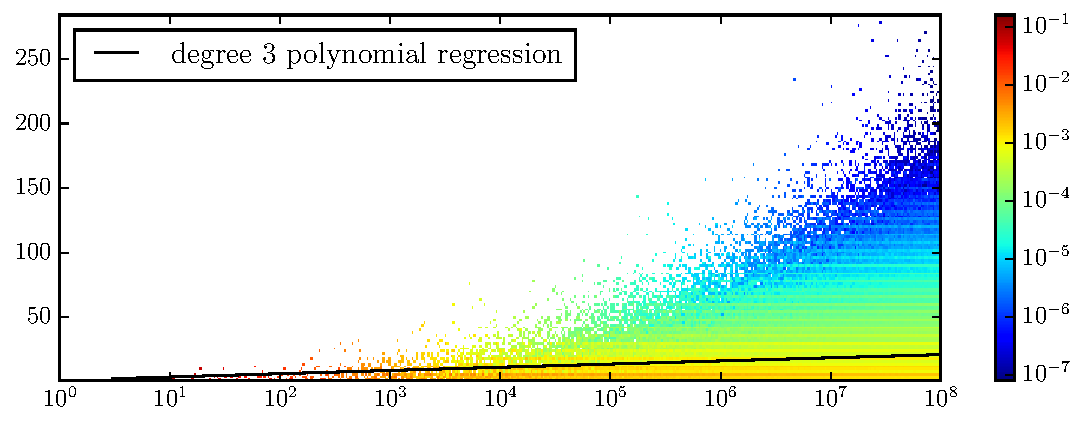
\includegraphics[width=\textwidth]{plots/arith_prog}
  \caption{Prime powers $r$ (abscissa) versus smallest integer $u$
    (ordinate) such that $ur+1$ is prime. Abscissa in logarithmic
    scale, density normalized by $\log(x)/x$ and colored in
    logarithmic scale.}
  \label{fig:primes-arith-prog}
\end{figure}

For the cyclotomic algorithm we also require that $\order_\ell(q)$ is
a multiple of $r$. Assuming that $q$ is uniformly
distributed\footnote{This assumption is obviously false for any fixed
  $q$, but it is a good enough approximation in practice.} in
$(\Z/\ell\Z)^\times$, its order is exactly $\ell-1$ with probability
$(\ell-1)/\ell$, hence we can assume that asymptotically
$\order_\ell(q)\in O(\ell)=O(r\log r)$. Similar considerations can be
made for the elliptic algorithm, assuming that $\ell\in
o(\sqrt[4]{q})$.
Finally, we must also take into account the possibility that the
elliptic algorithm fails. Under the heuristics of
Appendix~\ref{app:ellprdsdata}, this possibility only discards one in
$O(q^r)$ curves, and is thus negligible.


Summarizing, if we take $\bar{u},\bar{s}\in O(\log r)$, we can expect
Algorithm~\ref{algorithm:selectell} to find suitable parameters for
the cyclotomic algorithm, leading to expected parameters $\ell\in
O(r\log r)$, and to an expected running time of $\tildO(\sqrt{r})$
binary operations and $\tildO(\CC(r)+\MM(r)\log q)$ operations in
$\F_q$.  Similarly, if we also take $\bar{e}\in O(r\log r)$,
assuming that $r\log r\in o(\sqrt[4]{q})$, we can expect
Algorithm~\ref{algorithm:selectell} to find suitable parameters for
the elliptic algorithm, leading to an expected running time of
$\tildO(\sqrt{r}+(\log r)^2(\log q)^6)$ binary operations and
$\tildO(r^2\log q)$ operations in $\F_q$.

Although the complexity of the cyclotomic algorithm looks better, it
must not be neglected that the $\tildO$ notation
hides the cost of taking an auxiliary extension of degree
$O(\log r)$; whereas the elliptic algorithm, when it applies, does
not incur such overhead. The impact of the hidden terms in the
complexity can be extremely important, as we will show in the next
section. 

The same considerations also apply when comparing Rains' algorithms to
Allombert's. Indeed, the latter performs extremely well when the
degree $s$ of the auxiliary extension is small, but becomes slower as
this degree increases.

In practice, it is hopeless to try and determine the appropriate
bounds for each algorithm from a purely theoretical point of view. The
best approach we can suggest, is to determine parameters at runtime,
and set bounds and thresholds experimentally.
To summarize, given parameters $q$ and $r$, we suggest
the following approach:
\begin{enumerate}
\item If $\gcd(q,r)\ne 1$, run the Artin--Schreier algorithm of
  Section~\ref{sec:fast-artin-schreier}.
\item If $r$ is a power of a small prime $v$, run the algorithm of
  Section~\ref{sec:fast-algor-large}.
\item Determine the order $s$ of $q$ in $(\Z/r\Z)^\times$. If it is
  small enough, run one of the two variants of Allombert's algorithm
  presented in Section~\ref{sec:kummer}.
\item Run Algorithm~\ref{algorithm:selectell} with bounds $\bar{u}$,
  $\bar{s}$ and $\bar{e}$ determined according to $s$. Depending on
  the best parameters found by Algorithm~\ref{algorithm:selectell},
  run the best option among Rains' cyclotomic algorithm, Rains'
  elliptic algorithm, and Allombert's algorithm.
\end{enumerate}

In the next section we shall focus on the last two steps, by comparing
our implementations of the
algorithms involved, thus giving an estimate of the various thresholds
between them.  However we stress that these thresholds are bound to
vary depending on the implementation and the target platform, thus it
is the implementer responsibility to determine them at the moment of
configuring the system.

\begin{remark}
  Although our exposition focused on the case where $r$ is a prime
  power and $k\simeq K$, most of the algorithms presented here can be
  easily adapted to work more generally.

  In particular, it is a non-negligible practical improvement to work
  with composite $r$ by ``gluing'' together many prime powers. For
  example, let $r$ and $r'$ be two prime powers, and let $\ell$ and
  $\ell'$ be two primes selected for use in Rains' cyclotomic
  algorithm. If $\ell=\ell'$, then $\#\langle q\rangle=rr's$ for some
  $s$, and Rains' algorithm can be run only once for both $r$ and $r'$
  at the same time, with the added benefit of requiring a smaller
  auxiliary extension. Similarly, if $\ell\ne\ell'$, then we can run
  only once a straightforward generalization of Rains' algorithm using
  $(\ell\ell')$-th roots of unity; this is especially advantageous
  when $\order_\ell(q) = rs$ and $\order_{\ell'}(q) = r's$, so that
  the degree of the auxiliary extension is unchanged.

  In general, given the output of Algorithm~\ref{algorithm:selectell} for
  many prime powers, combining the results to obtain the best
  ``gluing'' requires solving an integer linear program (ILP). Given
  the availability of very fast ILP solvers, the practical speed-up
  can be significant.  Similar techniques also apply to Allombert's
  algorithm. On the other hand, it seems much more unlikely to apply
  them to the elliptic Rains' algorithm.
\end{remark}



\section{Experimental Results}
\label{sec:experimental-results}

To validate our results, we implemented the algorithms described in
the previous sections, and compared them to the implementation of
Allombert's algorithm available in Pari/GP~\cite{Pari}. The variants
of Allombert's algorithm described in Section~\ref{sec:fast-kummer}
were implemented in C on top of the Flint
library~\cite{hart2010flint}. Rains' cyclotomic and elliptic
algorithms were implemented in Sage~\cite{Sage} (which itself uses
Pari and Flint for representing finite fields), with critical code
rewritten in C/Cython (\todo{JP, do you want to give a better pointer
  to ellmul?}). Our code only handles $q$ prime and $m,n$ odd.

We ran tests for a wide range of primes $q$ between $5$ and
$2^{60}+3175$, and prime powers $r$ between $5$ and $1021$. All tests
were run on an Intel \todo{JP, what can you tell us?}. We report in
Figure~\ref{fig:bench} statistics only on the runs for
$2^{10}<q<2^{13}$; other ranges show very similar trends. The source
code and the full datasets can be downloaded at
\url{https://github.com/defeo/ffisom}.



\begin{figure}
  \newlength{\mywidth}
  \setlength{\mywidth}{8cm}
  \centering

  \begin{subfigure}{.48\textwidth}
    \includegraphics[width=\mywidth]{plots/bench-allombert-lowaux}
    \caption{Comparison of various implementations of Allombert's
      algorithm, in the case where the auxiliary degree
      $s=\order_q(r)\le 10$.  Dots represent individual runs, lines
      represent degree 2 linear regressions.}
    \label{fig:bench:allombert-lowaux}
  \end{subfigure}
  \hfill
  \begin{subfigure}{.48\textwidth}
    \noindent
    \includegraphics[width=\mywidth]{plots/bench-allombert-anyaux}
    \caption{Comparison of various implementations of Allombert's
      algorithm, as a function of the auxiliary degree
      $s=\order_q(r)$.  Individual running times are scaled by down by
      $r^2$.  Dots represent individual runs, lines represent degree 2
      linear regressions.}
    \label{fig:bench:allombert-anyaux}
  \end{subfigure}

  \begin{subfigure}{.48\textwidth}
    \noindent
    \includegraphics[width=\mywidth]{plots/bench-rains}
    \caption{Cyclotomic, conic and elliptic variants of Rains'
      algorithm.  Auxiliary extension degrees $s$ for cyclotomic
      Rains' range between $1$ and $9$.}
    \label{fig:bench:rains}
  \end{subfigure}
  \hfill
  \begin{subfigure}{.48\textwidth}
    \noindent
    \includegraphics[width=\mywidth]{plots/bench-all}
    \caption{Comparison of Allombert's and Rains' algorithms at some
      fixed auxiliary extension degrees $s$.}
    \label{fig:bench:all}
  \end{subfigure}

  \caption{Benchmarks for Rains' and Allombert's algorithms. $q$ is a
    prime between $2^{7}$ and $2^{13}$, $r$ is an odd prime power
    varying between $3$ and $509$.  Plots~\subref{fig:bench:rains}
    and~\subref{fig:bench:all} are in doubly logarithmic scale. Full
    dataset available at \url{https://github.com/defeo/ffisom}.}
  \label{fig:bench}
\end{figure}

In Figure~\ref{fig:bench:allombert} we compare the implementation of
Allombert's algorithm in Pari/GP with our own, specifically the
variant which is dubbed \emph{``case 2''} in
Section~\ref{sec:fast-kummer}. Each continuous line represents a batch
of runs of the cyclotomic variant with constant auxiliary degree
$s=\order_r(q)$, ranging from $1$ to $6$; runs with the same degree
$r$ are averaged together. In both implementations we observe a large
gap between $s=1$ and other values of $s$, due to the added cost of
computing in extension rings. While our variant performs better for
very small degree, it quickly catches and surpasses Pari in most
cases. However, our variant is considerably faster than Pari's when
the parameter $s$ gets larger, as we shall discuss in a few moments.

In Figure~\ref{fig:bench:rains} we compare the cyclotomic and elliptic
variants of Rains' algorithm. Each continuous line represents a batch
of runs of the cyclotomic variant with constant auxiliary degree
$s=\order_\ell(q)$, ranging from $1$ to $8$; runs with the same degree
$r$ are averaged together. Lines are clearly stacked on top of one
another according to their parameter $s$, only with occasional
crossings. We observe a very large gap between $s=1$ and larger $s$
($s=2$ is $8-16$ times slower). This is partly due to the fact that we
use generic Python code to construct auxiliary extensions, rather than
dedicated C; however a large gap is unavoidable, due to the added cost
of computing in extension fields. Dots represent individual runs of
the elliptic variant. We observe that on average it runs at a speed
which is intermediate between the cyclotomic variant with $s=2$ and
$s=3$. We wrote dedicated C code with optimized formulas for the
elliptic curve group operation, thus it seems difficult to improve the
gap between the elliptic and the cyclotomic variant. In conclusion the
cyclotomic variant only looks preferable to the elliptic one for very
small $s$, or when the elliptic variant does not apply.

To get a global view, we graph all algorithms in
Figure~\ref{fig:bench:all}. It appears that Allombert's algorithm
performs generally better than Rains' cyclotomic algorithm for small
auxiliary extension degree. Only when the $s$ parameter for
Allombert's algorithm reaches about $10$, it gets slower than Rains'
algorithm with $s=1$. The elliptic variant is even further up the
scale.

To more accurately determine the cross-points between the algorithms
we need to change picture. In Figure~\ref{fig:bench:allombert-vs-ell},
for every degree $r$ we compute the average running time of the
elliptic variant, then for each run of Allombert's algorithm (both in
Pari and in our version) we plot the ratio between its running time
and the average running time of the elliptic variant for the same
degree. We sort the ratios by increasing auxiliary extension degree
$s$ for Allombert's algorithm. It is then apparent that Pari's
implementation has a linear dependency in $s$, while our variant only
depends on it sub-linearly, as expected. This trend is even more
apparent with smaller primes $q$ and larger degrees $r$. The point
where both algorithms cross the elliptic variant of Rains' happens
around $s=100$. By postulating a constant ratio between Rains'
cyclotomic and elliptic variants, this graph can be used to determine
a cross-point for Allombert's \emph{versus} Rains' cyclotomic
algorithm too.

Obviously, these comparisons are only relevant to our own code and
test conditions. Other implementations and benchmarks will likely find
slightly different cross-points for the algorithms. Our goal here is
simply to show that all algorithms presented in this paper are
practical, that for each one there are specific parameters where it
performs best, and that our proposed variants constitute an
improvement over the state of the art.


%%%%%%%%%%%%%%%%%%%%%%%%%%%%%%%%%%
%%%%%%%%%%%%%%%%%%%%%%%%%%%%%%%%%%

\section{Embedding evaluation}
\label{sec:eval}

We end this work with a review of the known methods for
\emph{embedding evaluation}. %
We recall the problem statement: given two finite fields
$k=\F_q[X]/f(X)$ and $K=\F_q[Y]/g(Y)$, and given an embedding
$\phi:k\hookrightarrow K$ represented by two elements $\alpha\in k$
and $\beta\in K$ such that $k=\F_q(\alpha)$ and $\phi(\alpha)=\beta$,
answer the following questions:
\begin{itemize}
\item Given $\gamma\in k$, compute $\phi(\gamma)$;
\item Given $\delta\in K$, determine whether $\delta\in\phi(k)$;
\item Given $\delta\in\phi(k)$, compute
  $\phi^{-1}(\delta)$.\footnote{An additional natural question would
    be the following: given $\delta\in K$, compute an expression
    $\delta=\sum_{i=0}^{n/m-1} \phi(\gamma_i) Y^i$ with all
    $\gamma_i\in k$. The techniques presented here also apply to this
    more general problem, however we will skip them for conciseness.}
\end{itemize}
We are going to assume that elements of $k$ are represented on the
monomial basis $(1,X,\dots,X^{m-1})$, and elements of $K$ on the
monomial basis $(1,Y,\dots,Y^{n-1})$.

We review three solutions for this problem, each built on top
of the previous one. %
The first one uses basic linear algebra; it is simple and effective,
but has large space and time complexities. %
The second one improves the complexity by avoiding matrix inversion;
however it is still based on linear algebra, thus it has the same
storage requirements as the previous method. %
The last one replaces linear algebra with modular composition, thus
providing the best space and time complexities overall. 

All the methods presented in this section are classic and well
understood, thus we will keep the presentation short, and will not
discuss implementation details.

\subsection{Linear algebra}
\label{sec:linear-algebra}

Since the map $\phi$ is $\F_q$-linear, one obvious solution is to
explicitly write its matrix on the monomial bases of $k$ and $K$. %
This is the solution employed by both the PARI/GP~\cite{Pari} and the
Magma~\cite{MAGMA,bosma+cannon+steel97} computer algebra systems. %
To stress the fact that $k$ is seen a vector space with a fixed basis
$(1,X,\dots,X^{m-1})$, we will write $V_X$ for it, and we will
similarly write $V_Y$ for $K$ with its monomial basis. %

The element $\alpha$ defines another basis
$(1,\alpha,\dots,\alpha^{m-1})$ of $k$, and we denote by $V_\alpha$
this vector space isomorphic to $V_X$. %
Similarly, $\beta$ defines a basis of a subspace $V_\beta\subset V_Y$,
also isomorphic to $V_\alpha$. %
Hence, we decompose the map $\phi:V_X\to V_Y$ as a composition of
three maps:
\[V_X \xrightarrow{\;\sim\;} V_\alpha \xrightarrow{\;\sim\;} V_\beta \lhook\joinrel\longrightarrow
  V_Y.\] %
The middle map from $V_\alpha$ to $V_\beta$ is trivially represented
by an identity matrix; the only maps that require actual computation
are the other two. %

For example, the map $V_\beta\hookrightarrow V_Y$ is represented by an
$n\times m$ matrix whose columns are the coefficients of the elements
$1,\beta,\dots,\beta^{m-1}$ written on the monomial basis of $V_Y$. %
The inverse map is then computed by solving a linear system; this
operation can be sped up by precomputing, e.g., an LU decomposition
for the matrix. %
The computation of the map $V_X\xrightarrow{\sim}V_\alpha$ is done
analogously.

Summarizing, both the full map $\phi:V_X\to V_Y$ and its inverse can
be computed by performing one matrix-vector product and solving one
linear system. %
The complexity is dominated by the cost of solving the linear system,
that is $O(m^{\omega-1}n)$ operations over $\F_q$. %
However this cost can be counted as a precomputation if we perform an
LU decomposition, and so can the computation of the powers $\alpha^i$
and $\beta^i$; in this case, the cost for evaluating $\phi$ or its
inverse drops down to $O(mn)$ operations. %
At any rate, the biggest drawback of this approach is the large memory
complexity: indeed storing the precomputed matrices requires $O(mn)$
elements of $\F_q$.

\subsection{Inverse maps and duality}

The first improvement to the linear algebraic method consists in
replacing the linear system solving with a much simpler matrix-vector
product, combined with an efficient change of basis. %
This technique is not
new~\cite{shoup94,shoup95,shoup99,bostan+salvy+schost03}, however it
is seldom found in the literature. %
We briefly recall it, following the presentation of~\cite{DeDoSc2014}.

Let $k=\F_q[X]/f(X)$ be a finite field with monomial basis
$(1,X,\dots,X^{m-1})$. %
The trace $\trace$ from $k$ to $\F_q$ defines a non-degenerate
bilinear form by
$\ang{\gamma,\delta}_k \equiv \trace(\gamma\delta)$,
which itself determines the \emph{dual basis}
$(X_0^*,X_1^*,\dots,X_{m-1}^*)$ to $(1,X,\dots,X^{m-1})$,
characterized by
\begin{equation*}
  \ang{X^j,X_i^*}_k = \begin{cases}
    1 &\text{if $i=j$,}\\
    0 &\text{otherwise.}
  \end{cases}
\end{equation*}
Given the polynomial $f$, conversions between the monomial and the
dual basis can be performed very efficiently at a cost of
$O(\MM(m)\log m)$ operations in $\F_q$ (see~\cite[\S~3]{DeDoSc2014}).

Let now $K=\F_q[Y]/g(Y)$ be another finite field, let $\ang{,}_K$ be
the bilinear form defined by its trace to $\F_q$, and let
$\phi:k\hookrightarrow K$ be a field embedding. %
There exists a unique linear map $\phi^t:K\to k$, called the
\emph{dual map} of $\phi$, such that
\begin{equation*}
  \ang{\phi(\gamma),\delta}_K=\ang{\gamma,\phi^t(\delta)}_k
  \qquad\text{for any $\gamma\in k$ and $\delta\in K$.}
\end{equation*}
If $M=(m_{i,j})$ is the matrix of $\phi$ in the monomial bases of $k$
and $K$, then its transpose $M^t$ is the matrix of $\phi^t$ in their
\emph{dual bases}. %
Indeed,
\begin{equation}
  \label{eq:tellegen-matrix}
  m_{i,j} = \ang{\phi(X^j),Y_i^*} = \ang{X^j,\phi^t(Y_i^*)}.
\end{equation}

We are now going to show that $\phi^t$ is closely related to the
inverse map of $\phi$. %
If $\phi$ is an isomorphism of fields, then we immediately have
$\phi^t=\phi^{-1}$. %
Indeed, in this case $\phi$ preserves the bilinear forms:
\begin{equation*}
  \ang{\gamma,\delta}_k = \ang{\phi(\gamma),\phi(\delta)}_K
  \qquad\text{for any $\gamma,\delta\in k$.}
\end{equation*}
Hence, duality implies that
\begin{equation*}
  \ang{\gamma,\delta}_k = \ang{\gamma,\phi^t\circ\phi(\delta)}_k,
\end{equation*}
but then the non-degeneracy of the trace implies that
$\phi^t\circ\phi$ is the identity map.\footnote{More generally, in the
  category of finite-dimensional vector spaces with nondegenerate
  bilinear forms and morphisms that preserve bilinear forms, we have a
  natural isomorphism between the identity functor and the dual
  functor.}

The case where $\phi$ is a proper embedding calls for a more careful
handling. %
In this case, $\phi$ does not preserve traces, indeed, if $n=[K:\F_q]$,
\begin{equation*}
  \frac{n}{m}\ang{\gamma,\delta}_k = \ang{\phi(\gamma),\phi(\delta)}_K.
\end{equation*}
If $n/m$ is not a multiple of the characteristic, proceeding like
before we can show that $(m/n)\phi^t$ is the inverse of $\phi$. %
To handle the general case, take an element $\eta\in K$ such that
$\trace_{K/k}(\eta)=1$, and let $H$ be the map defined by
$\gamma\mapsto\eta\gamma$. %
Then, by composition of traces, we prove that
\begin{equation*}
  \ang{\gamma,\delta}_k = \trace_{k/\F_q}(\gamma\delta) =
  \trace_{K/\F_q}(\gamma\eta\delta) = \ang{\phi(\gamma),H\circ\phi(\delta)}_K =
  \ang{H\circ\phi(\gamma),\phi(\delta)}_K 
\end{equation*}
We have thus shown that both $\phi^t\circ H\circ\phi$ and
$\phi^t\circ H^t\circ\phi$ are the identity map.

Let us apply these findings to the linear algebraic approach of the
previous subsection. %
We had an embedding of fields, decomposed as three maps
\[V_X \xrightarrow{\;\sim\;} V_\alpha \xrightarrow{\;\sim\;} V_\beta
  \lhook\joinrel\longrightarrow V_Y.\] %
The maps $V_\alpha\xrightarrow{\sim} V_X$ and
$V_\beta\hookrightarrow V_Y$ are both field embeddings; the first one
is represented by its matrix on the monomial bases generated by
$\alpha$ and $X$; the second one on those generated by $\beta$ and
$Y$. %
For both maps, we are interested in computing their inverse; instead
of solving a linear system, we switch to dual bases and apply the
discussion above. %
Thus, the inverse of $V_\beta\hookrightarrow V_Y$ is evaluated as a
multiplication by a fixed element $\eta$, followed by a conversion to
the dual basis of $V_Y$, then a matrix-vector product with the
transposed matrix, and finally a conversion back to the monomial basis
of $V_\beta$. %
The inverse of $V_\alpha\xrightarrow{\sim}V_X$ is computed similarly. %

Note that the inverse map to $V_\beta\hookrightarrow V_Y$ is not
everywhere defined. %
Interestingly, while linear system solving could immediately recognize
elements of $V_Y$ that are not in the image of $V_\beta$, the new
solution will just project them onto an arbitrary element of
$V_\beta$. %
Indeed, any $\delta\in V_Y$ can be rewritten as
\begin{equation*}
  \delta = (\delta - \trace_{K/k}(\eta\delta)) + \trace_{K/k}(\eta\delta)
  = \delta' + \trace_{K/k}(\eta\delta),
\end{equation*}
for the same $\eta$ chosen above. %
Direct calculation shows that
\begin{equation}
  \label{eq:projection}
  \ang{\phi(\gamma),\eta\delta}_K =
  \ang{\phi(\gamma),\eta\delta'}_K + \ang{\phi(\gamma),\eta\trace_{K/k}(\eta\delta)}_K =
  \ang{\gamma, \trace_{K/k}(\eta\delta)}_k,
\end{equation}
for any $\gamma\in k$. %
Hence, applying the above algorithm to an arbitrary element
$\delta\in V_Y$ yields the element $\trace_{K/k}(\eta\delta)$ of
$V_\beta$, which coincides with $\delta$ whenever
$\delta\in\phi(k)$. %
Hence, the best way to test that an element $\delta\in K$ is in the
image of $\phi$ would be to project it to
$\gamma=\trace_{K/k}(\eta\delta)$ using this algorithm, and then test
that $\phi(\gamma)=\delta$.

It is easily seen that the complexity is dominated by the transposed
matrix-vector product, which costs $O(mn)$ operations (plus a cost of
$O(m\MM(n))$ operations for precomputing the matrices). %
Hence, by paying a little overhead in the changes of basis, we have
completely removed the cost of solving a linear system. %
We have not reduced yet the large storage cost, however.


\subsection{Modular composition}

Our final improvement consists in replacing the matrix computations
with modular composition. %
The technique originates in Shoup's
work~\cite{shoup94,shoup95,shoup99}.

Considering again the map $V_\beta\hookrightarrow V_Y$, we observe
that its evaluation is precisely a modular composition problem: given
polynomials $\gamma=\sum \gamma_i\beta^i$ and $\beta=\sum \beta_iY^i$
with coefficients in $\F_q$, of degree bounded by $n$, compute
$\gamma(\beta)\bmod g$. %
As seen previously this computation can be done more efficiently by a
dedicated algorithm, than by a naive Horner rule.

However we also need to compute the inverse map to
$V_\beta\hookrightarrow V_Y$, and this problem is clearly not a
modular composition one. %
In the previous subsection we have reduced the computation of this
inverse map to a change of bases, combined with a transposed
matrix-vector product. %
A very powerful generalization of Eq.~\eqref{eq:tellegen-matrix},
called \emph{transposition principle}, allows us to \emph{transpose}
any modular composition algorithm, much like one would transpose a
matrix. %
This technique was also introduced by Shoup, and then refined by many
authors~\cite{bostan+lecerf+schost:tellegen,df+schost10,df+thesis}. %
The \emph{dual problem} to modular composition was named \emph{power
  projection} by Shoup; its inputs are the polynomials $\beta,g$, and
an element $\gamma^*$ in the dual space of $\F_q[X]$ (i.e., the linear
forms on $\F_q[X]$); its output is the list of elements
$\gamma^*(\beta^0),\dots,\gamma^*(\beta^{n-1})$. %
Thanks to the transposition principle, the power projection problem
can be solved in the same complexity as modular
composition~\cite{shoup95,kedlaya+umans08}.

Summarizing, the inverse map to $V_\beta\hookrightarrow V_Y$, is
computed by Algorithm~\ref{alg:inv-mod-comp}.

\begin{algorithm}
    [Inverse embedding]
    \label{alg:inv-mod-comp}
    \begin{algorithmic}[1]
      \REQUIRE An element $\delta\in K$, and precomputed values:\\
      $\bullet\;\beta\in K$ generating a subfield isomorphic to $k$,\\
      $\bullet\;\eta\in K$ such that $\trace_{K/k}\eta=1$.
      \ENSURE $\trace_{K/k}(\eta\delta)$ written in the basis $(1,\beta,\dots,\beta^{m-1})$.
      \STATE Compute the minimal polynomial of $\beta$ over $\F_q$;
      \STATE Compute $\delta'=\eta\delta$;
      \STATE Convert $\delta'$ to the dual basis $(Y_0^*,\dots,Y_{n-1}^*)$;
      \STATE Compute $\gamma=\trace_{K/k}\delta'$ using \emph{power projection};
      \STATE Convert $\gamma$ to the monomial basis $(1,\beta,\dots,\beta^{m-1})$;
      \RETURN $\gamma$.
    \end{algorithmic}
\end{algorithm}

\begin{theorem}
  Algorithm~\ref{alg:inv-mod-comp} is correct. %
  When the input $\delta$ is in the image of $k$, it returns $\delta$
  itself written on the basis $(1,\beta,\dots,\beta^{m-1})$. %
  It computes its output using $O(\CC(n))$ operations in $\F_q$.
\end{theorem}
\begin{proof}
  Correctness follows from the discussion above, and the obvious fact
  that $\delta=\trace_{K/k}(\eta\delta)$ whenever $\delta\in k$.

  The minimal polynomial of $\beta$, required to compute conversions
  between the monomial and the dual bases generated by $\beta$, can be
  computed in $O(\MM(n)\log n)$ operations using the Berlekamp--Massey
  algorithm.\footnote{The minimal polynomial could be precomputed
    along with $\beta$, however we include this computation in the
    algorithm, as it does not change the total complexity.} %
  Conversions between monomial and dual bases are also done in
  $O(\MM(n)\log n)$ as shown in~\cite[\S~3]{DeDoSc2014}. %
  Finally, the power projection costs $O(\CC(n))$ operations, using
  any of the algorithms in~\cite{shoup95,kedlaya+umans08}.
\end{proof}

We have not specified how the element $\eta$ is computed. %
If $n/m$ is not divisible by the characteristic, then one can simply
take $\eta=m/n$. %
In the general case, it suffices to know an element such that
$\trace_{K/k}\ne0$, and to divide it by its trace. %
If the $(n-1)$-th coefficient of $g$ is not $0$, then $Y$ is one such
element; otherwise we take elements at random until a suitable one is
found: only $O(1)$ trials are expected on average. %
In any case, computing one trace can be done using
$O(\CC(n)\log(n)+\MM(n)\log(q))$ operations, thanks to
Proposition~\ref{prop:trace-like}.

\begin{corollary}
  After a precomputation costing $O(\CC(n)\log(n)+\MM(n)\log(q))$
  operations in $\F_q$ on average, all sub-questions of the
  \emph{embedding evaluation problem} can be answered using
  $O(\CC(n))$ operations in $\F_q$.
\end{corollary}



\appendix
\part*{Appendices}
\addcontentsline{toc}{part}{Appendices}

%%%%%%%%%%%%%%%%%%%%%%%%%%%%%%%%%%

\section{More variants of Rains' algorithm}
\label{app:rains-vars}

We have seen that Rains' cyclotomic algorithm suffers in practice from
the need to build a field extension $k'$ of $k$. %
In this section we present two variants of Rains' algorithm that help
reduce the cost associated to the field extension. %
None of the two variants has an impact on the overall complexity of
Rains' algorithm.

\paragraph{Rains' conic algorithm}
The first variant reduces the degree of the field extension from
$s=[k':k]$ to $s/2$ whenever $s$ is even. %
This is especially useful when $s=2$, as highlighted in
Section~\ref{sec:experimental-results}. %
The algorithm is similar in spirit to Williams' $p+1$ factoring
method~\cite{williams1982}, where the arithmetic of the norm $1$
subgroup of ${k'}^*$ is performed using Lucas sequences on a subfield
of index $2$ of $k'$.

Let $\F$ be a finite field of odd characteristic, let $\Delta\in\F$ be
a quadratic non-residue, let $\delta$ be an element of the algebraic
closure of $\F$ such that $\delta^2=\Delta$, and define the norm $1$
subgroup of $\F[\delta]^*$ as
\[T_2(\F) = \{(x+\delta y)/2 \;\mid\; x,y\in\F \text{ and } x^2-\Delta
  y^2 = 4\};\] %
it is easy to verify that $T_2(\F)$ forms a group under
multiplication. %
If we see the elements $(x+\delta y)/2$ as points $(x,y)$ on a conic
$x^2-\Delta y^2=4$, the group law of $T_2(\F)$ induces a group law on
the conic. %
By projecting onto the $x$-coordinate, a straightforward calculation
shows that, for any point $(\theta,*)$ on the conic, its $n$-th power
has coordinates $(\theta_n,*)$, where $\theta_n$ is defined by the
Lucas sequence
\[\theta_0 = 2, \quad \theta_1 = \theta, \quad \theta_{i+1}=\theta\theta_i-\theta_{i-1}.\] %
We shall denote by $[n]$ the map $\theta\mapsto\theta_n$; notice how
it does not depend on the choice of $\Delta$.

The generalization of Rains' algorithm is now obvious: by projecting
on the $x$-coordinate, we work in a field extension twice as small
compared to the original algorithm. %
This is summarized in Algorithm~\ref{algorithm:rains-conic}.

\begin{algorithm}[Rains' conic algorithm]
  \label{algorithm:rains-conic}
  \begin{algorithmic}[1]
    \REQUIRE A field extension $k/\F_q$ of degree $r$; a prime $\ell$
    such that
    \begin{itemize}
    \item $(\Z/\ell\Z)^\times = \langle q\rangle \times S$ for some $S$,
    \item $\#\langle q\rangle = 2rs$ for some integer $s$;
    \end{itemize}
    a polynomial $h$ of degree $s$ irreducible over $k$.
    \ENSURE A normal generator of $k$ over $\F_q$,
    with a uniquely defined Galois orbit.
    
    \STATE Construct the field extension $k'=k[Z]/h(Z)$;
    \REPEAT
    \REPEAT
    \STATE Take a random element $\theta\in k'$,
    \UNTIL\label{algorithm:rains-conic:sqtest} $\theta^2-4$ is a quadratic non-residue;
    \STATE\label{algorithm:rains-conic:power} Compute $\zeta=[(\#k'+1)/\ell]\theta$,
    \UNTIL $\zeta\ne2$;
    \STATE\label{algorithm:rains-conic:period} Compute $\eta(\zeta) \leftarrow \sum_{\sigma\in S}[\sigma]\zeta$;
    \RETURN\label{algorithm:rains-conic:trace} $\alpha \leftarrow \trace_{k'/k}\eta(\zeta) = \sum_{i=0}^{s-1}[q^{ri}]\eta(\zeta)$.
  \end{algorithmic}
\end{algorithm}

\begin{proposition}
  Algorithm~\ref{algorithm:rains-conic} is correct: on input
  $q,r,\ell,s$ it returns an element in the same Galois orbit as
  Algorithm~\ref{algorithm:rains-cyclo} on input $q,r,\ell,2s$. %
  It computes its output using $O(\MM(sr)(sr\log q+(\ell/r)\log\ell))$
  operations in $\F_q$ on average, or $\tildO((sr)^2\log q)$ assuming
  $\ell\in o(sr^2)$.
\end{proposition}
\begin{proof}
  By construction, all the $\ell$-th roots of unity are in
  $T_2(k')$. %
  Observe that if $(x+\delta y)/2$ is in $T_2(k')$, then its trace
  over $k'$ is equal to $x$. %
  Hence, the value $\zeta$ computed in
  Step~\ref{algorithm:rains-conic:power} is the trace over $k'$ of a
  primitive $\ell$-th root of unity. %
  We conclude by comparing this algorithm with
  Algorithm~\ref{algorithm:rains-cyclo}.

  The non-residuosity test in Step~\ref{algorithm:rains-conic:sqtest}
  is done by verifying that the $(\#k'-1)/2$-th power of $\theta$ is
  equal to $-1$. %
  We do this in $O(sr\log q)$ operations in $k'$, or
  $O(sr\MM(sr)\log q)$ operations in $\F_q$.

  To implement the other steps, we need to evaluate the map $[n]$
  efficiently. %
  We have the following classical relationships for the Lucas sequence
  of $\theta$:
  \begin{equation*}
    \theta_{2i} = \theta_{i}^2-2,\quad
    \theta_{2i+1} = \theta_i\theta_{i+1} - \theta,\quad
    \theta_{2i+2} = \theta_{i+1}^2-2.
  \end{equation*}
  Starting with $\theta_0=2$ and $\theta_1=\theta$, we use a binary
  scheme to deduce $\theta_i,\theta_{i+1}$ from
  $\theta_{\lfloor i/2\rfloor},\theta_{\lfloor i/2\rfloor+1}$. %
  We reach $\theta_n$ after $O(\log n)$ steps, each requiring a
  constant number of operations in $k'$.

  Hence, Step~\ref{algorithm:rains-conic:power} costs
  $O(sr\MM(sr)\log(q))$ operations in $\F_q$, while
  Steps~\ref{algorithm:rains-conic:period}
  and~\ref{algorithm:rains-conic:trace} together cost
  $O((\MM(sr)\ell\log\ell)/r)$.
\end{proof}

Although this variant does not exploit the asymptotic improvement
offered by Proposition~\ref{prop:large-power}, the fact that its
auxiliary degree $s$ is half the one of the original algorithm usually
gives an interesting practical improvement. %
Step~\ref{algorithm:rains-conic:power} can be modified so as to avoid
the premature projection on the $x$-axis, so that the algorithm of
Proposition~\ref{prop:large-power} applies. %
We leave the details of this variant to the reader.


\paragraph{Rains' cyclotomic algorithm without auxiliary polynomials}
Our second variant avoids the construction of the field extension $k'$
altogether by factoring the cyclotomic polynomial $\Phi_\ell$, thus
eliminating the need for a precomputed list of irreducible
polynomials. In the algorithm below we denote by $[\bar{h}]_i$ the
degree $i$ coefficient of the polynomial $\bar{h}$.

\begin{algorithm}[Rains' cyclotomic algorithm variant]
  \label{algorithm:rains-cyclo-2}
  \begin{algorithmic}[1]
    \REQUIRE A field extension $k/\F_q$ of degree $r$, a prime $\ell$ such that
    \begin{itemize}
    \item $(\Z/\ell\Z)^\times = \langle q\rangle \times S$ for some $S$,
    \item $\#\langle q\rangle = rs$ for some integer $s$.
    \end{itemize}
    \ENSURE A normal generator of $k$ over $\F_q$,
    with a uniquely defined Galois orbit.
    
    \STATE Compute a factor $h$ of the $\ell$-th cyclotomic polynomial $\Phi_\ell$ in $k[Z]$; 
    \STATE Compute $\bar{h} \leftarrow -\frac{h'(1/Z)}{Zh(1/Z)} \bmod Z^\ell$;
    \RETURN $\alpha \leftarrow \sum_{\sigma\in S}[\bar{h}]_\sigma$.
  \end{algorithmic}
\end{algorithm}


\begin{proposition}
  Algorithm~\ref{algorithm:rains-cyclo-2} is correct. %
  On input $q,r,\ell,s$ it computes its output using
  $O(\ell r(\log(s)+\log(r))\log(\ell) + \MM(\ell r)\log(\ell r) +
  \MM(\ell r)\log(q))$ operations in $\F_q$ on average, or
  $\tildO(\ell r\log (q))$.
\end{proposition}
\begin{proof}
  Let $\zeta$ be the image of $Z$ in $k[Z]/h(Z)$. Obviously $\zeta$ is
  an $\ell$-th root of unity. By Newton's identities, we have the
  equality of power series
  \begin{equation*}
    -\frac{h'(1/Z)}{Zh(1/Z)} = \sum_{i>0}\sum_{j=0}^{s-1}(\zeta^i)^{q^{rj}} Z^i.
  \end{equation*}
  Hence, summing the $\sigma$-th coefficients in the above series for
  $\sigma\in S$ gives the sought period.

  The complexity is dominated by the cost of factoring $\Phi_\ell$,
  that is
  $O(\ell r(\log(s)+\log(r))\log(\ell) + \MM(\ell r)\log(\ell r) +
  \MM(\ell r)\log(q))$ operations according to
  Proposition~\ref{prop:cyclo}. Indeed, the computation of $\bar{h}$
  costs only $O(\MM(\ell r))$ operations, and the final sum
  $O(\ell r)$ operations.
\end{proof}

By comparing the latter algorithm with Rains' original one, we see
that this variant performs better when $s$ is larger than $r$. %
Although we were unable to prove that this cannot be the case, we saw
in Section~\ref{sec:selection} that $s$ is typically in
$O(\log(r))$. %
Furthermore, the algorithms of Section~\ref{sec:kummer} always have
better complexity than this one. %
Thus this latter variant of Rains' algorithms seems to be of purely
theoretical interest.


%%%%%%%%%%%%%%%%%%%%%%%%%%%%%%%%%%

\section{Elliptic curves}
\label{app:elliptic-curves}


% Another subtlety arises in comparison with multiplicative groups:
% elliptic curves always come with non trivial automorphisms. We recall
% that the size of the \emph{group of rational automorphisms} of a curve
% $E/\F_q$ is one of the following:
% \begin{itemize}
% \item $\#\Aut_{\F_q}(E) = 12$ if $j(E)=0$ and $q=0\mod 9$ \todo{is this correct? useful?},
% \item $\#\Aut_{\F_q}(E) = 6$ if $j(E)=0$ and $q=1\mod 3$,
% \item $\#\Aut_{\F_q}(E) = 4$ if $j(E)=1728$ and $q=1\mod 4$,
% \item $\#\Aut_{\F_q}(E) = 2$ otherwise.
% \end{itemize}


Recall that two elliptic curves $E$ and $E'$ over a field $k$ are said
to be \emph{isomorphic} if there exists a linear change of variables
with coefficients in $k$ sending one onto the other. If $E$ and $E'$
are isomorphic over $\bar{k}$, but not over $k$, they are said to be
\emph{twists} of each other. A twist is said to be quadratic
(resp. cubic, quartic, sextic), if $E$ and $E'$ become isomorphic over
a quadratic (resp. cubic, quartic, sextic) extension of $k$. Most
elliptic curves only have quadratic twists; elliptic curves with
$j=0,1728$ may have cubic, quartic and sextic twists. See~\cite{Sil}.

We now give a proposition relating the number of points of an elliptic
curve over a finite field with the number of points of its twists.  In
the case of quadratic twists, this proposition simply states that $E$
and $E'$ have opposite trace, a well known fact.

\begin{proposition}
  \label{proposition:twisttrace}
  Let $E$ be an ordinary elliptic curve defined over a finite field
  $\F_q$ of characteristic $p\ne2$, and denote by $t$ the trace of its
  Frobenius endomorphism.

  Let $u\in\bar{\F}_q$, define a curve $E^u$ and an isomorphism
  $\upsilon$ of elliptic curves by
  \begin{equation*}
    \begin{aligned}
      \upsilon : E &\to E^u,\\
      (x,y) &\mapsto (u^2x,u^3y).
    \end{aligned}
  \end{equation*}
  If $E^u$ is defined over $\F_q$, then $u^{q-1}$ is an element of
  $\F_p$ of multiplicative order $n\in\{1,2,3,4,6\}$.

  Let $t_u$ be the trace of the Frobenius endomorphism of $E^u$, then
  $t_u^n=t^n \bmod q$, and $t_u=u^{q-1}t\bmod p$. This is enough to
  uniquely determine $t_u$ given $t$.
\end{proposition}
\begin{proof}
  Observe that if $E^u$ is a quadratic (resp. cubic, quartic, sextic)
  twist of $E$, then $u^{q-1}$ has multiplicative order $2$
  (resp. $3,4,6$). Furthermore, since $E$ is ordinary, $2$
  (resp. $3,4,6$) divides $p-1$, hence $u^{q-1}$ is in the prime field
  $\F_p$, and it defines a curve automorphism
  \begin{equation*}
    \upsilon^{q-1}:(x,y)\mapsto(u^{2q-2}x,u^{3q-3}y).
  \end{equation*}
  Any twist arises this way (see~\cite{Sil}).

  Denote by $\pi$ and $\pi_u$ the frobenius endomorphisms of $E$
  and $E^u$ respectively. They satisfy the equations
  \begin{equation}
    \label{eq:frob-char-twist}
    \pi^2 - [t]\pi + [q] = 0, \qquad \pi_u^2 - [t_u]\pi_u + [q] = 0,
  \end{equation}
  where $[m]$ denotes multiplication by $m$ on the elliptic curves. By
  straightforward calculation, we also verify that they satisfy the
  commutative diagram
  \begin{equation*}
    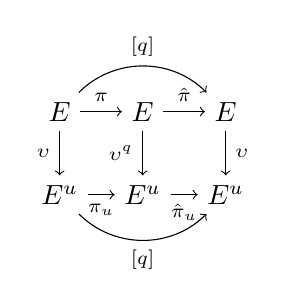
\begin{tikzpicture}[node distance=3em]
      \node(E){$E$};
      \node[right of=E](E2){$E$};
      \node[right of=E2](E3){$E$};
      \node[below of=E](Eu){$E^u$};
      \node[right of=Eu](Eu2){$E^u$};
      \node[right of=Eu2](Eu3){$E^u$};

      \draw[->,auto,font=\scriptsize]
      (E) edge node[swap]{$\upsilon$} (Eu)
          edge node{$\pi$} (E2)
          edge[bend left=45] node{$[q]$} (E3)
      (Eu) edge node[swap]{$\pi_u$} (Eu2)
           edge[bend right=45] node[swap]{$[q]$} (Eu3)
      (E2) edge node[swap]{$\upsilon^q$} (Eu2)
           edge node{$\hat\pi$} (E3)
      (Eu2) edge node[swap]{$\hat\pi_u$} (Eu3)
      (E3) edge node{$\upsilon$} (Eu3);
    \end{tikzpicture}
  \end{equation*}
  where we denote by $\upsilon^q$ the isomorphism
  $(x,y)\mapsto(u^{2q}x,u^{3q}y)$, and by $\hat\pi,\hat\pi_u$ the dual isogenies
  to $\pi,\pi_u$.

  Now we restrict the maps above to the $q$-torsion subgroups of $E$
  and $E^u$. Since the curves are ordinary, these subgroups are cyclic
  of order $q$, and the maps act as scalar multiplication on the
  points. In particular, we deduce from Eq.~\eqref{eq:frob-char-twist} that 
  \begin{equation*}
    \pi = [t \bmod q], \qquad \pi_u = [t_u \bmod q].
  \end{equation*}
  Hence, from the diagram we obtain
  \begin{equation*}
    [t] = \upsilon^{-q}\circ[t_u]\circ\upsilon \mod q.
  \end{equation*}

  Notice that $\upsilon^{-q}$ can be decomposed as
  $\upsilon^{-1}\circ\upsilon^{1-q}$, where $\upsilon^{1-q}$ is an
  automorphism of $E^u$ by hypothesis. $\upsilon^{1-q}$ also acts on
  the $q$-torsion points as a scalar in $\Z/q\Z$, that we shall denote
  by $U$. It is evident that the multiplicative order of $U$ in $\Z/q\Z$
  is the same as that of $u^{1-q}$ in $\F_p$. Then
  \begin{equation*}
    [t] = \upsilon^{-1}\circ[Ut_u]\circ\upsilon\mod q.
  \end{equation*}
  But $\upsilon$ is an isomorphism, thus it commutes with scalar
  multiplication, and we conclude that $t=Ut_u\bmod q$.

  If $u^{1-q}=\pm1$, we are done. When the order of $u^{1-q}$ is $3,4$
  or $6$, we still have to determine which of the cubic, fourth, sixth
  roots of unity in $\Z/q\Z$ corresponds to $U$.

  Using the diagram above, we decompose
  Eq.~\eqref{eq:frob-char-twist} as
  \begin{equation*}
    \hat\pi\circ\pi = [t]\pi - \pi^2,
  \end{equation*}
  and similarly for $E^u$. Hence, from the diagram again,
  \begin{equation}
    \label{eq:twisttrace:modp}
    [t] - \pi = \hat\pi = \upsilon^{-1}\circ\hat\pi_u\circ\upsilon^q 
    =  \upsilon^{-1}\circ([t_u] - \pi_u)\circ\upsilon^q.
  \end{equation}
  Let now $\omega$ be the invariant differential of $E$, we apply the
  pullback of Eq.~\eqref{eq:twisttrace:modp} to $\omega$. On the
  left-hand side we have
  \begin{equation}
    \label{eq:twisttrace:modp-lhs}
    ([t]-\pi)^\ast\omega = t\omega\in\Omega_E
  \end{equation}
  because $\pi$ is inseparable (see \cite[\S~5]{Sil}). On the
  right-hand side, if we let $\omega_u$ be the invariant differential
  of $E^u$, we have $(\upsilon^{-1})^\ast\omega=u\omega_u$, and
  $(\upsilon^q)^\ast\omega_u=\omega/u^q$, hence
  \begin{equation}
    \label{eq:twisttrace:modp-rhs}
    (\upsilon^{-1}\circ([t_u] - \pi_u)\circ\upsilon^q)^\ast\omega =
    u(([t_u] - \pi_u)\circ\upsilon^q)^\ast\omega_u =
    ut_u(\upsilon^q)^\ast\omega_u = u^{1-q}t_u\omega.
  \end{equation}
  Comparing Eqs.~\eqref{eq:twisttrace:modp-lhs}
  and~\eqref{eq:twisttrace:modp-rhs}, we conclude that $t = u^{1-q}t_u
  \bmod p$. Given that $\lvert t_u\rvert\le2\sqrt{q}$, we have uniquely determined $t_u$, and proven the theorem.
\end{proof}

\todo{Give a similar proposition for supersingular curves (see, e.g.,
  Menezes--Okamoto--Vanstone)}

\section{Elliptic periods}
\label{app:ellprdsdata}

In this section, we discuss theoretical and experimental aspects
of the validity of Conjecture~\ref{conj:ellperiods}:
elliptic periods provide polynomial bases of finite fields.

\subsection{Heuristic arguments}

A natural idea to prove this conjecture would be to transpose
the proof that cyclotomic periods do generate bases of finite fields.
Unfortunately, as far as cyclotomic periods are concerned,
the only proof we are aware of proceeds as follows.
For a squarefree $\ell$ and $q = p$ prime:
\begin{enumerate}
\item the $\ell$-th cyclotomic polynomial is irreducible over $\Q$ and
a primitive $\ell$-root of unity $\zeta_\ell$ yield a normal basis
of $\Q(\zeta_\ell)$;
\item Gaussian periods seen as field traces of roots of unity
then yield normal bases of subextensions;
\item integrality properties of these bases for $p \neq \ell$
and picking up a subextension where $p$ is inert show that
the situation transposes to characteristic $p$ by reduction.
\end{enumerate}
The second step of the proof crucially relies on the normality
of the bases generated by cyclotomic bases and, as we know
that elliptic periods do not generate normal bases,
there is little hope to transpose this proof to elliptic periods.
Moreover, this suggests that, if a proof exists for elliptic periods,
it does not involve lifting to characteristic zero
and takes place in positive characteristic only.
Therefore, the polynomially cyclic algebras setting of \cite{Mihailescu2010825}
looks like a reasonable approach to attempt such a proof.
Although we were unsuccessful to do so, working whithin this setting gives
heuristic arguments that, even though it is not a general fact,
elliptic periods often yield normal bases.

\paragraph{Polynomially cyclic algebras}
Let $f_\lambda$ be the kernel polynomial of the isogeny corresponding
to the eigenspace of $\lambda$ and $A$ be the (polynomially cyclic)
algebra
\[
A = \F_q[x]/(f_\lambda(x)) \; .
\]

By hypothesis $\lambda$ is of order $r$ modulo $q$ so that
the kernel polynomial $f_\lambda$ splits as
\[
f_\lambda = h_1 \cdots h_d
\]
where the $h_i$ are pairwise coprime irreducible polynomial of degree $r$
(and $d r = (l-1)/2$).
Therefore the algebra $A$ splits as
\[
A \simeq \F_q[x]/(h_1(x)) \times \cdots \times \F_q[x]/(h_d(x)) \; .
\]
The $h_i$ correspond to the different Galois orbits of the abscissae
of the eigenpoints of $\lambda$.

Let $c$ be a generator of $(\Z/\ell\Z)^{\times}/\{\pm 1\}$.
The multiplication-by-$c$ map on $E$ cyclicly permutes the
abscissae of the eigenpoints of $\lambda$ and
induces a cyclic automorphism $\nu$ of the algebra $A$.
Up to permutation of indices, we can suppose that $\nu$
sends roots of $h_i$ onto roots of $h_{i+1}$.
Let $C$ be the sole polynomial of degree less than $(l-1)/2$
describing $\nu$ on $A$ (that is the one obtained by taking the
rational fraction expressing multiplication-by-$c$ and inverting
its denominator modulo $f_\lambda$).
Given a polynomial $g$ representing an element of $A$, note that
$\nu$ acts by composing $g$ with $C$: $\nu(g) = g(C)$.

Recall that
$(\Z/\ell\Z)^{\times}/\{\pm 1\} = \langle{\lambda}\rangle \times S$
and let $s = c^r$ be a generator of $S$.
We denote by $\sigma$ the automorphism of algebra $\nu^{(r)}$
and by $S$ the corresponding polynomial
(there should be no confusion with the subgroup $S$).
Note that $\nu^d$ is the Frobenius automorphism of $A$.

Gathering the above remarks we obtain the following diagram:
\begin{center}
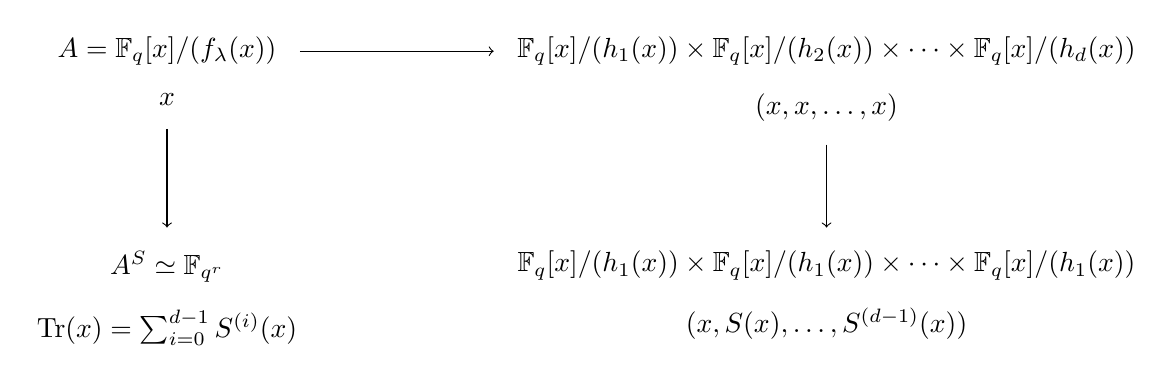
\begin{tikzpicture}
\node (A) {$A=\F_q[x]/(f_\lambda(x))$};
\node[below=.3em of A] (Ax) {$x$};
\node[right=8em of A] (CRT) {$\F_q[x]/(h_1(x)) \times \F_q[x]/(h_2(x)) \times \cdots \times \F_q[x]/(h_d(x))$};
\node[below=.3em of CRT] (CRTx) {$(x, x, \ldots, x)$};
\node[below=6em of A] (T) {$A^S \simeq \F_{q^r}$};
\node[below=.3em of T] (Tx) {$\mathrm{Tr}(x) = \sum_{i = 0}^{d-1} S^{(i)}(x)$};
\node[below=6em of CRT] (C) {$\F_q[x]/(h_1(x)) \times \F_q[x]/(h_1(x)) \times \cdots \times \F_q[x]/(h_1(x))$};
\node[below=.3em of C] (Cx) {$(x, S(x), \ldots, S^{(d-1)}(x))$};
\draw[->, shorten >= .5em, shorten <= .5em] (A) -- (CRT);
\draw[->, shorten >= .5em, shorten <= .5em] (Ax) -- (T);
\draw[->, shorten >= .5em, shorten <= .5em] (CRTx) -- (C);
\end{tikzpicture}
\end{center}

\begin{proposition}
\label{prop:xnormal}
If $x \in A$ is a normal element,
then $\eta_{\lambda,S}(P)$ is a normal element in $\F_{q^r}$
for any eigenpoint $P$ of $\lambda$.
\end{proposition}

\begin{proof}
Suppose that $x$ is normal in $A$, then so is its trace in $A^S$.
But taking the trace of $x$ in $A$ and going through the two isomorphisms
of the diagram is the same thing as computing the period in the
$d$ different representations of $\F_{q^r}$:
\[
x \mapsto \sum_{i=0}^{d-1} S^{(i)}(x) \mapsto
\left( \sum_{i=0}^{d-1} S^{(i)}(x) \pmod{h_1(x)}, \ldots,
\sum_{i=0}^{d-1} S^{(i)}(x) \pmod{h_d(x)} \right) \; .
\]
If a linear relation existed between $\eta_{\lambda,S}(P) \in \F_q(x(P))$
and its Galois conjugates for any eigenpoint $P$ of $\lambda$,
it would be verified in the $d$ different representations of $\F_{q^r}$
and lift up to $A$ implying the same linear relation for
$\mathrm{Tr}(x)$ and its Galois conjugates.
Therefore, if $x$ is normal in $A$,
then $\eta_{\lambda,S}(P)$ is normal in $\F_q(x(P))$.
\end{proof}

The converse is easily shown not to be true by experimentation.
There is also no relation between the normality of $x \in A$
and $x(P) \in \F_q(x(P))$ for any eigenpoint $P$ of $\lambda$,
or between the normality of $x(P)$ and that of $\eta_{\lambda,S}(P)$.

Nonetheless, Proposition~\ref{prop:xnormal} shows that heuristically
$\eta_{\lambda,S}(P)$ has a high probability to be normal and therefore
to generate $\F_q(x(P))$.
Indeed, supposing that $x \in A$ behaves as a random element
as far as normality is concerned, it has a high probability
of begin normal, just as random elements in finite fields,
as the following lemma shows.
\begin{lemma}
\label{lemma:euleralgebra}
Let $A$ be a polynomially cyclic algebra of degree $dr$
over the finite field $\F_q$.
The number of normal elements in $A$ is the same as the
number of normal elements in $\F_{q^{dr}}$:
$\Phi_q(x^{dr}-1) \in O(q^{dr})$ where $\Phi_q$ is the Euler function
for polynomials~\cite[Lemma~3.69]{lidl+niederreiter:2}.
\end{lemma}
\begin{proof}
There is at least one normal element in $A$~\cite[Theorem 4]{Mihailescu2010825}
(and it can be constructed from one in $\F_q$).
One such element $\alpha$ can be used to count the number of normal elements
as in the finite field case~\cite[Theorem~3.73]{lidl+niederreiter:2}:
\begin{enumerate}
\item every element $a$ can be written using the normal basis
associated to $\alpha$: $a = \sum_{i=0}^{dr-1} a_i \nu^{(i)}(\alpha)$;
\item as the Galois group of $A$ is cyclic, the decomposition
of the Galois conjugates of $a$ is obtained by shifting the coefficients $a_i$;
\item the circulant matrix $M_a$ associated to the $a_i$'s is invertible
if and only if $a$ is a normal element;
\item the polynomial $\sum_{i=0}^{dr-1} a_i x^i$ in $\F_q[x] / (x^{dr}-1)$
is invertible if and only if $M_a$ is.
\end{enumerate}
Therefore normal elements in $A$ are in one-to-one correspondence
with units of $\F_q[x] / (x^{dr}-1)$.
\end{proof}

\paragraph{Further heuristics}
Another heuristic argument supporting the fact that
elliptic periods should generate $\F_{q^r}$
(at least when $q$ and $r$ are prime, although it can be adapted to
a more general setting) follows:
considering that $\eta_{\lambda, S}(P)$ behaves as a random
element of $\F_{q^r}$, the probability that it does not
generate $\F_{q^r}$, or equivalently that it lies in
the only strict subfield of $\F_{q^r}$ which is $\F_q$,
is $q^{1-r}$.
Therefore, counterexamples should be seeked for small values
of $q$ and $r$, but as stated in the following section,
we found none so far.

To conclude this theoretical discussion, note that one might be tempted to
replace the trace above by any symmetric function of the
Galois conjugates of $x \in A$ such as the norm.
In the case of cyclotomic Gaussian periods,
replacing the trace by the norm either gives another root of unity
when the computation is trivial, or $1$ when it is not,
so such an operation has no sense.
But in the case of elliptic periods, there is no reason to expect such a
phenomenon.
However for most elementary symmetric functions, except for the trace,
couterexamples were found by small scale experiments.

\subsection{Searching for counterexamples}

We now present experimental evidence supporting the validity of
Conjecture~\ref{conj:ellperiods}.
As discussed above, if counterexamples to the conjecture
are to be found, they should be seeked
for small values of $q$ and $r$ as the probability that a random element
does not generate $\F_{q^r}$ is expected to decrease as $q^{-r}$.

\paragraph{Search strategy 1}
For small values of $q$,
one can generate random elliptic curves over $\F_q$,
look for small values of $l$ which are Elkies primes,
compute a point of $l$-torsion defined over $\F_{q^r}$,
the associated elliptic period and its minimal polynomial.

If one restricts to prime values of $q$ and $r$ and supposes elements
of $\F_{q^r}$ are represented as polynomials with coefficients in $\F_q$,
the computation of the minimal polynomial can be avoided:
one simply checks that the elliptic period is not in $\F_q$,
i.e. a constant polynomial.

\paragraph{Search strategy 2}
With further restrictions on $r$ and $\ell$ it is possible to avoid
the computation of an actual $\ell$-torsion point as well.
For example, let $r$ be a prime such that $\ell = 2 d r + 1$
with $d = 2$ is prime
and suppose that $l$ is an Elkies prime for $E$:
the $\ell$-division polynomial $f_\ell$ of $E$ has two factors
$h_1$ and $h_2$ of degree $r$ over $\F_{q}$
(whose product is $f_\lambda$).
The elliptic period is defined as $x(P) + x([i] P)$ for some
$i \in \left(Z / \ell \Z\right)^*$ such that $i^2 \equiv -1 \pmod{\ell}$
and any $P \in E(\F_{q^r})[\ell]$.
Let $m_i$ be multiplication by $i$ map on the curve.
Then the mapping $x + m_i(x)$ sends the roots of $h_1$
and the roots of $h_2$ onto the ellptic periods.
If we suppose that the period is not generating $\F_{q}$ which implies that
$\Res_x(h_1(x),y-x-m_i(x)) = \Res_x(h_2,y-x-m_i(x))$
splits over $\F_{q}$,
then by Galois invariance $x + m_i(x) \equiv t \pmod{h_1}$
for a constant $t \in \F_{q}$,
and since the periods do not depend on the initial choice of $h_1$
or $h_2$,
we conclude that $m_i(x) \equiv (t-x) \pmod{h_1 h_2}$.
Hence, we can just compute $x + m_i(x) \pmod{h_1 h_2}$
and see if it is a constant.
The dominating step in this approach is the factorization of $f_\ell$.
For large values of $q$ it could be replaced by using modular polynomials
and isogeny computations \`a la SEA, but the chances of finding counterexamples
are higher for small $q$'s and this would give no practical improvement.
Such an approach can easily be generalized to larger values of $d$.

\paragraph{Search strategy 3}
Finally, one can apply the above approach in a global way:
pick a rational elliptic curve and known to have a rational $\ell$-isogeny
and $\ell$-torsion over an extension of degree $r$ (or $2r$)
with $\ell = 2 d r + 1$,
then compute the kernel polynomial of the isogeny
$f_\lambda = h_1 \ldots h_d$ with $h_1, \ldots, h_d$ of degree $r$ 
and check that there is no prime outside those of bad reduction or
with reduction equipped with more than a couple of automorphisms
dividing all the coefficients, except possibly the constant one, of
$x + m_i(x) + \ldots + (m_i \circ \cdots \circ m_i) (x) \pmod{h_k}$,
where $k$ is any index and $i$ a $d$-th root of $-1$ in
$\left(Z / \ell \Z\right)^*$.

For $r=3$, $d = 2$ and $\ell = 2 d r + 1 = 13$,
there are infinitely many such curves
and they all belong to a parametrized family
exhibited by Daniels et al.~\cite{daniels_torsion_2015} with $j$-invariant:
\[
j(t)=\frac{\left(t^4-t^3+5 t^2 + t + 1\right) \left(t^8 - 5 t^7 + 7 t^6 - 5 t^5 + 5 t^3 + 7 t^2 + 5 t + 1\right)^3}{t^{13} \left(t^2 -3 t - 1\right)} \enspace .
\]
%Among them is is curve~\texttt{147b1} in Cremona's table~\cite{cremona_tables}.
In practice, the limiting step of this method is computing the $j$-invariant
of the curves because its height quickly grows.

The next candidate for prime $r$ and $\ell$, and $d = 2$, can not be used.
Indeed, for $r = 7$ and $\ell = 29$, there is no rational elliptic curve
with a rational $29$-isogeny~\cite{Mazur1974} (or elliptic curves defined
over a septic number field with $29$-torsion~\cite{Derickx201452}).
More generally, rational elliptic  curves with rational $\ell$-isogenies
exist only for a finite set of values of $\ell$ corresponding
to non-cuspidal rational points on $X_0(\ell)$, leaving few chances
to find other interesting curves.

Among the suitable prime values for $\ell \geq 13$~\cite{Mazur1974},
only $\ell = 13$ provides an infinite family parametrized~\cite{Lozano-Robledo2013} by
\[
j(t) = \frac{\left(t^2 + 5t + 13\right)\left(t^4 + 7t^3 + 20t^2 + 19t + 1\right)^3}{t} \enspace .
\]
Within this family are the aforementioned curves
with $13$-torsion defined over a cubic extension.
For $\ell = 17, 19, 163$, the factorizations of $(\ell-1)/2 = 2^3, 3^2, 3^4$
do not allow coprime values for $d$ and $r$.
For $\ell = 37$, there is a couple of rational elliptic curves with a rational
$37$-isogeny.
The first one is \texttt{1225H1} in Cremona's tables~\cite{cremona_tables}
%with $j$-invariant $-7\cdot11^3$
% $37$-torsion$ is defined over an extension of $\Q$ of degree $(\ell-1)/3 = 12$
and its kernel polynomial splits into three factors of degree $6$
leaving no possibility for coprime $d$ and $r$ as $3$ must divide $d$
and $2$ can not divide $r$.
The other one is \texttt{1225H2} in Cremona's tables~\cite{cremona_tables}
%with $j$-invariant $-7\cdot137^3\cdot2083^3$
and its kernel polynomial $f_\lambda$ is irreducible.
For each $\ell = 43, 67$, there is exactly one rational elliptic curve
with a rational $\ell$-isogeny,
and the corresponding kernel polynomials $f_\lambda$ are both irreducible.
The factorization of $(\ell-1)/2$ leaves the possibility to define
coprime values for $d$ and $r$ although the irreducibility of $f_\lambda$
limits the probability of a splitting into $d$ factors modulo $p$ even
if one finds a $p$ as above.

A few composite values of $\ell$ for which rational elliptic curves
with a rational $\ell$-isogeny can also be considered.
The first value for $\ell$ is $\ell = 21$, with $\phi(21) = 2\cdot2\cdot3$.
There are exactly four rational elliptic curves with a rational $21$-isogeny
labeled \texttt{162b1}, \texttt{162b2}, \texttt{162b3}, and \texttt{162b4}.
All of them have a rational point of $3$-torsion.
The elliptic curve~\texttt{162b1} is the unique elliptic curve
with $21$-torsion over a cubic extension of $\Q$~\cite{najman_cubic},
and indeed its  kernel polynomial factorizes into one linear factor
and three cubic factors.
For the three other curves, the kernel polynomial factor into
one linear factor, one cubic and one sextic.
One can therefore use $d=2$ and $r=3$ in this case.
The second value for $\ell$ is $\ell = 25$, with $\phi(25) = 2\cdot2\cdot5$.
In this case there is an infinity of rational elliptic curves
with a rational $25$-isogeny parametrized\cite{Lozano-Robledo2013} by
\[
j(t) =
\frac{\left(t^{10}+10t^8+35t^6-12t^5+50t^4-60t^3+25t^2-60t+16\right)^3}
{t^5+5t^3+5t-11}\enspace .
\]
There is also an infinity of elliptic curves defined over a quintic
extension $K$ of $\Q$ with $25$-torsion defined over
$K$~\cite{Derickx201452,2016arXiv160807549D}.
If one of these curves is actually defined over $\Q$,
it has rational $5$-torsion~\cite{gonzalez-jimenez_complete_2016}.
Parametrizing such curves is outside the scope of this work,
but one can still sample curves within the larger family
and compute periods for $d=2$ and $r=5$.
Note that in this case, $25$ is not squarefree,
so one should compute periods using the more general formula
from~\cite{feisel1999normal}.
The third value for $\ell$ is $\ell = 27$, but $\phi(27) = 2\cdot3^2$,
and there are no suitable coprime values for $d$ and $r$.

\paragraph{Experimental results}
All above strategies were implemented and ran on different ranges of parameters.

For strategy 1, for different ranges of $\ell$ we tested all elliptic curves
defined over $\F_q$ with $q$ prime up to some bounds
and such that $\ell$ is an Elkies prime with an eigenvalue
of prime order $r$ (without any bound on $r$).
The greatest $q$ tested are given in Table~\ref{table:strat1}.
\begin{figure}[!ht]
\[
\begin{array}{|*{6}{c|}}
\hline
\ell & [0, 100] & [100, 200] & [200, 300] & [300, 400] & [400, 500] \\
\hline
q_{\max} & 4957 & 2767 & 2063 & 1171 & 983 \\
\hline
\hline
\ell & [500, 600] & [600, 700] & [700, 800] & [800, 900] & [900, 1001] \\
\hline
q_{\max} & 467 & 1283 & 503 & 271 & 419 \\
\hline
\end{array}
\]
\caption{Largest value of $q$ tested for a given range of $\ell$ with strategy 1.}
\label{table:strat1}
\end{figure}

For strategy 2, we picked up small values of $r$ and $\ell = 2 \cdot 2 \cdot r + 1$
and checked all elliptic curves defined over $\F_q$ with $q$ prime up
to some bound.
The greatest $q$ tested are given in Table~\ref{table:strat1}.
\begin{figure}[!ht]
\[
\begin{array}{|*{6}{c|}}
\hline
r & 3 & 7 & 13 & 37 & 43 \\
\hline
q_{\max} & & & & & \\
\hline
\end{array}
\]
\caption{Largest value of $q$ tested for a given $r$ with strategy 2.}
\label{table:strat2}
\end{figure}

For strategy 3, we tested all rational values of $t$
with numerator and denominator of absolute values less than $10000$.

No counter-example was found.
%%%%%%%%%%%%%%%%%%%%%%%%%%%%%%%%%%
%%%%%%%%%%%%%%%%%%%%%%%%%%%%%%%%%%

\bibliographystyle{plain}
\bibliography{refs}

\end{document}


% Local Variables:
% ispell-local-dictionary:"american"
% End:

%  LocalWords:  isomorphism cyclotomic coprime subfield Frobenius
%  LocalWords:  endomorphism eigenspace Allombert's polynomially
%  LocalWords:  automorphism morphism morphisms
